\documentclass[11pt,]{article}
\usepackage{lmodern}
\usepackage{amssymb,amsmath}
\usepackage{ifxetex,ifluatex}
\usepackage{fixltx2e} % provides \textsubscript
\ifnum 0\ifxetex 1\fi\ifluatex 1\fi=0 % if pdftex
  \usepackage[T1]{fontenc}
  \usepackage[utf8]{inputenc}
\else % if luatex or xelatex
  \ifxetex
    \usepackage{mathspec}
  \else
    \usepackage{fontspec}
  \fi
  \defaultfontfeatures{Ligatures=TeX,Scale=MatchLowercase}
\fi
% use upquote if available, for straight quotes in verbatim environments
\IfFileExists{upquote.sty}{\usepackage{upquote}}{}
% use microtype if available
\IfFileExists{microtype.sty}{%
\usepackage{microtype}
\UseMicrotypeSet[protrusion]{basicmath} % disable protrusion for tt fonts
}{}
\usepackage[margin=1in]{geometry}
\usepackage{hyperref}
\PassOptionsToPackage{usenames,dvipsnames}{color} % color is loaded by hyperref
\hypersetup{unicode=true,
            pdftitle={Yellow Rail in Alberta's Oil Sands Region},
            pdfauthor={Richard Hedley, Marcus Becker, Erin Bayne},
            colorlinks=true,
            linkcolor=blue,
            citecolor=Blue,
            urlcolor=Blue,
            breaklinks=true}
\urlstyle{same}  % don't use monospace font for urls
\usepackage{longtable,booktabs}
\usepackage{graphicx,grffile}
\makeatletter
\def\maxwidth{\ifdim\Gin@nat@width>\linewidth\linewidth\else\Gin@nat@width\fi}
\def\maxheight{\ifdim\Gin@nat@height>\textheight\textheight\else\Gin@nat@height\fi}
\makeatother
% Scale images if necessary, so that they will not overflow the page
% margins by default, and it is still possible to overwrite the defaults
% using explicit options in \includegraphics[width, height, ...]{}
\setkeys{Gin}{width=\maxwidth,height=\maxheight,keepaspectratio}
\IfFileExists{parskip.sty}{%
\usepackage{parskip}
}{% else
\setlength{\parindent}{0pt}
\setlength{\parskip}{6pt plus 2pt minus 1pt}
}
\setlength{\emergencystretch}{3em}  % prevent overfull lines
\providecommand{\tightlist}{%
  \setlength{\itemsep}{0pt}\setlength{\parskip}{0pt}}
\setcounter{secnumdepth}{5}
% Redefines (sub)paragraphs to behave more like sections
\ifx\paragraph\undefined\else
\let\oldparagraph\paragraph
\renewcommand{\paragraph}[1]{\oldparagraph{#1}\mbox{}}
\fi
\ifx\subparagraph\undefined\else
\let\oldsubparagraph\subparagraph
\renewcommand{\subparagraph}[1]{\oldsubparagraph{#1}\mbox{}}
\fi

%%% Use protect on footnotes to avoid problems with footnotes in titles
\let\rmarkdownfootnote\footnote%
\def\footnote{\protect\rmarkdownfootnote}

%%% Change title format to be more compact
\usepackage{titling}

% Create subtitle command for use in maketitle
\providecommand{\subtitle}[1]{
  \posttitle{
    \begin{center}\large#1\end{center}
    }
}

\setlength{\droptitle}{-2em}

  \title{Yellow Rail in Alberta's Oil Sands Region}
    \pretitle{\vspace{\droptitle}\centering\huge}
  \posttitle{\par}
    \author{Richard Hedley, Marcus Becker, Erin Bayne}
    \preauthor{\centering\large\emph}
  \postauthor{\par}
      \predate{\centering\large\emph}
  \postdate{\par}
    \date{October 18, 2019}

\usepackage{float}

\begin{document}
\maketitle

{
\hypersetup{linkcolor=black}
\setcounter{tocdepth}{4}
\tableofcontents
}
\clearpage

\section{Introduction}\label{introduction}

Yellow Rails (\emph{Coturnicops noveboracensis}) are one of the most
secretive and poorly understood bird species in North America. They are
migratory, spending the months of May until September at their breeding
grounds throughout Canada, and the rest of the year in wetlands along
the southeast coast of the United States. The remoteness of their
wetland breeding habitats and their nocturnal activity patterns render
them poorly sampled by standard bird monitoring efforts. A lack of
information regarding distribution, population size, population trends,
and basic biology has been a primary reason for conservation concern.
The purpose of this report is to summarize findings from monitoring
efforts in the Oil Sands Region (OSR) of Alberta, synthesize available
knowledge into tools for future management, and highlight priorities for
further research.

\begin{figure}[H]

{\centering 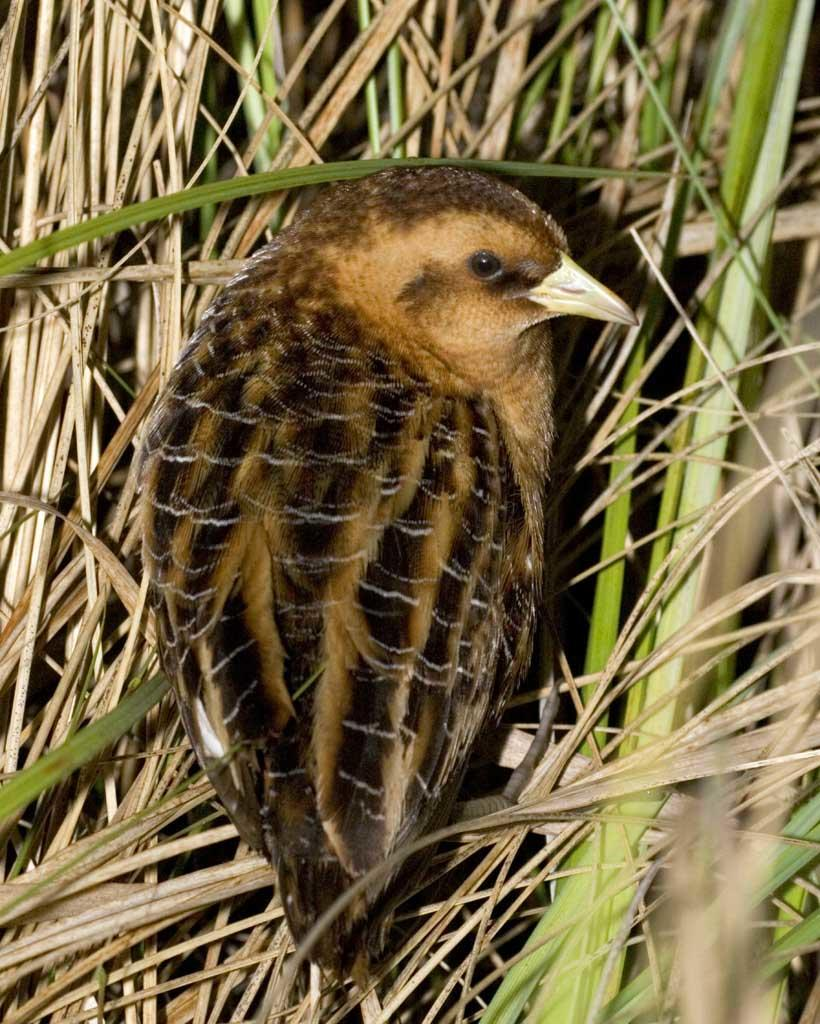
\includegraphics[width=0.4\linewidth]{C:/Users/mabec/Documents/R/OSM-Synthesis-YERA/./docs/pics/yellow-rail} 

}

\caption{Yellow Rail. Photo credit  Audobon Society.}\label{fig:yera-pic}
\end{figure}

\subsection{At Issue}\label{at-issue}

Current knowledge of the breeding habits of Yellow Rails suggests that
they primarily breed in graminoid fens, with breeding territories
characterized by 0 to 30-cm of standing water and dense cover of grasses
and sedges (Stenzel, 1982; Bookhout and Stenzel, 1987; Austin and Buhl,
2013; Leston and Bookhout, 2015). Much of this breeding territory is in
remote areas of the boreal natural region (Wells and Blancher, 2011).

The two main threats facing the Yellow Rail in the OSR are:

\begin{itemize}
\tightlist
\item
  the \textbf{direct effects} of surface mining, in which their habitats
  are removed;
\item
  the \textbf{indirect effects} of altered hydrology due to development,
  which may affect the suitability of habitat well beyond the footprint
  of development (Environment Canada, 2013).
\end{itemize}

\subsection{Management Goals}\label{management-goals}

Yellow Rail abundance and occupancy can fluctuate from year to year at a
wetland, which is thought to be driven by inter-annual variation in
water levels. Nevertheless, some wetlands in the OSR are reliably
occupied by large numbers of Yellow Rails every year (dozens of
individuals, E.Bayne \emph{unpublished}). As such, a management goal for
this species in the OSR is to identify Yellow Rail breeding sites and
prioritize these for conservation. As part of this, monitoring must be
focused on understanding both the direct and indirect effects of
development on key habitats, such as the mineable regions around
McClelland Lake (as required by the Environmental Protection and
Enhancement Act).

\section{Monitoring and Research
Objectives}\label{monitoring-and-research-objectives}

\begin{itemize}
\tightlist
\item
  \textbf{Identify key breeding sites}
\end{itemize}

Currently, Yellow Rails have been found at approximately 200 survey
points in the OSR. A habitat map constructed from these data can be used
to predict additional breeding sites and estimate population sizes and
potential threats. Predicted sites should be surveyed when possible to
verify presence/absence. Regions that are potentially important but
which have not been thoroughly surveyed include the wetlands surrounding
Lake Clair in Wood Buffalo National Park, the entire ``western
panhandle'' of the OSR, and most wetlands not within 10-km of a road.

Identification of new sites can be accomplished by visiting sites of
high predicted habitat suitability to confirm presence/absence of Yellow
Rails. In particular, visiting areas with large expanses of predicted
suitable habitat is important, as these locations are likely to harbour
significant populations of Yellow Rails.

\begin{itemize}
\tightlist
\item
  \textbf{Refine population estimates}
\end{itemize}

Existing population estimates put the population of Yellow Rail at
10,000 - 25,000 individuals globally. The population in Alberta has been
estimated at 500 pairs. However, this is likely an underestimate,
because recent surveys have found nearly 300 males (with an assumed
equal number of females) in the surveyed areas of the OSR, which itself
covers only about 20\% of the province (E.Bayne, unpublished data). The
degree of underestimation remains unknown and is the focus of ongoing
work. In this report we present preliminary results from Hedley et al.
(\emph{in prep}) that report a new regional population estimate for the
species based on monitoring from 2013-2018.

\begin{itemize}
\tightlist
\item
  \textbf{Continue research on movement ecology}
\end{itemize}

Yellow Rails migrate from Canada to the southeastern United States each
year. Beyond this, little is known about their movements. The consensus
view regarding the conservation of migratory species is that successful
conservation efforts must focus on the full annual cycle.

Populations in Quebec are thought to undertake a molt migration in the
late summer, moving dozens of kilometers from their breeding grounds to
molt. It is not known if Yellow Rails in Alberta do the same, but if
they do, it may mean their habitat needs extend well beyond their
breeding territories.

Yellow Rails are also notorious for their lack of site fidelity. Rates
of recapture of the same individual in successive years are
\textless{}1\% (K. Drake, Pers. Comm.), suggesting that the rails move
around between years. This behaviour is thought to have evolved as an
adaptation to ephemeral wetland habitats, which can become unsuitable if
water levels are too high or too low. The low (\textless{}1\%)
interannual recapture rate is a practical barrier to long-distance
tracking, since most tracking devices require recapture. Those that
remotely transmit data via satellite are currently too large to attach
to Yellow Rails. An intermediate option is a GPS tag with the option of
data download via short-range radio receivers, and this option is
currently being explored.

\begin{itemize}
\tightlist
\item
  \textbf{Assess threats posed in the OSR}
\end{itemize}

Several oil sands mines (or proposed mines) abut or overlap significant
patches of potential Yellow Rail habitat. Research is ongoing to place
these threats within regional and global contexts. This is proceeding in
two main ways: first, by continuing to survey suitable habitat on and
near leases to determine if the predicted habitat is actually occupied;
and second, by estimating the percentage of predicted habitat that
occurs on, near, and off lease, and using these percentages to estimate
proportion of the regional and global population that are threatened by
development. Additionally, existing water depth data will be used to
examine how Yellow Rails respond to changes in water levels between
years, and findings can be used to develop better mitigation strategies.

\begin{itemize}
\tightlist
\item
  \textbf{Develop tools for Yellow Rail management}
\end{itemize}

Finally, research findings can be distilled into tools for land managers
to improve Yellow Rail conservation in the future. In this report we
present a predictive habitat suitability map (30-m raster resolution)
that can be used to assess threats to Yellow Rail in the region and
identify new potential breeding sites.

\section{Data Collection}\label{data-collection}

The status of Yellow Rails in the oilsands region has been poorly
understood historically because they are not well surveyed by standard
monitoring efforts. In 2012, the now-defunct Ecological Monitoring
Committee for the Lower Athabasca began targeted surveys for Yellow
Rails throughout the oilsands region. In the first year, human point
counts and autonomous recording units (ARUs) were both employed in
surveys, but it was quickly determined that ARUs are as good or better
than humans at detecting Yellow Rails, and have the added benefit that
they do not require humans to venture to remote areas at night. ARUs
have been the sole survey method since 2013.

Yellow Rails are surveyed through listening to recordings made at 2:00am
during peak breeding season, which runs from roughly May 20 to July 15
each year. At 2:00am, we have found that Yellow Rails are highly vocal
and easily detected, such that a 1-minute survey has a
\textasciitilde{}50\% probability of detecting a Yellow Rail, given that
one is present. Therefore, at each station surveyed in a given year,
four 2:00am recordings are listened to to detect the presence of rail.
The four recordings are randomly sampled from the available days between
June 1 and July 15. Conducting multiple surveys per station allows
estimation of both occupancy rate and detection probability via
occupancy analysis (discussed in the results section below).

Just 2 Yellow Rails were detected at 302 survey stations in 2012 (0.007
individuals per sation); these findings initiated an iterative process
whereby detections were used to refine our understanding of habitat
preferences, which was then used to identify additional sites to survey.
As evidence of the effectiveness of this process, at 102 stations that
were visited for the first time in 2018 and had high predicted
suitability, we found 22 Yellow Rail individuals (0.22 individuals per
station, more than 30 times the rate of detections in 2012).

Once a wetland has been selected for surveys, multiple ARUs are usually
placed within the wetland. The most common deployment scheme is to place
five ARUs in a square with 600m edges: one unit is placed at each
corner, and one in the middle. Variations on this theme have been used,
with the general intent of placing ARUs sufficiently far
(\textgreater{}500m) from their nearest neighbours to increase spatial
independence. Each ARU placement is considered a `site' in the analysis
below, and displayed on the map.

In addition to visiting new sites, we have resurveyed previous survey
locations, which will allow an assessment of inter-annual variation in
site occupancy and analysis of trends over time. As of 2018, 143 survey
stations with at least one Yellow Rail detection had been surveyed in
multiple years.

\section{Results}\label{results}

\subsection{Key Breeding Sites in the
OSR}\label{key-breeding-sites-in-the-osr}

We set out to identify and monitor key Yellow Rail breeding sites in the
OSR, as per our first objective. Figure \ref{fig:survey-sites} below
displays the location of sites surveyed for Yellow Rail between
2013-2018. Seven regionally important wetlands (or wetland complexes)
are listed in Table \ref{fig:wetlands}, and are the source of 249 of 286
(87\%) of the individual males detected from 2013 to 2018 via acoustic
surveys. The Eastern and Western McClelland Fen Mine sites, represented
by the cluster of sites north of Fort McMurray, have together produced
118 (41\%) detections over the period surveyed. No other wetland site
has so far been found to contain more than 10 individuals. For smaller
wetlands, the number of detected males may represent a reasonable
population estimate of males at the wetland; however, for larger
wetlands where only a portion of the wetland has been sampled, this is
likely an underestimate.

\begin{figure}[H]

{\centering 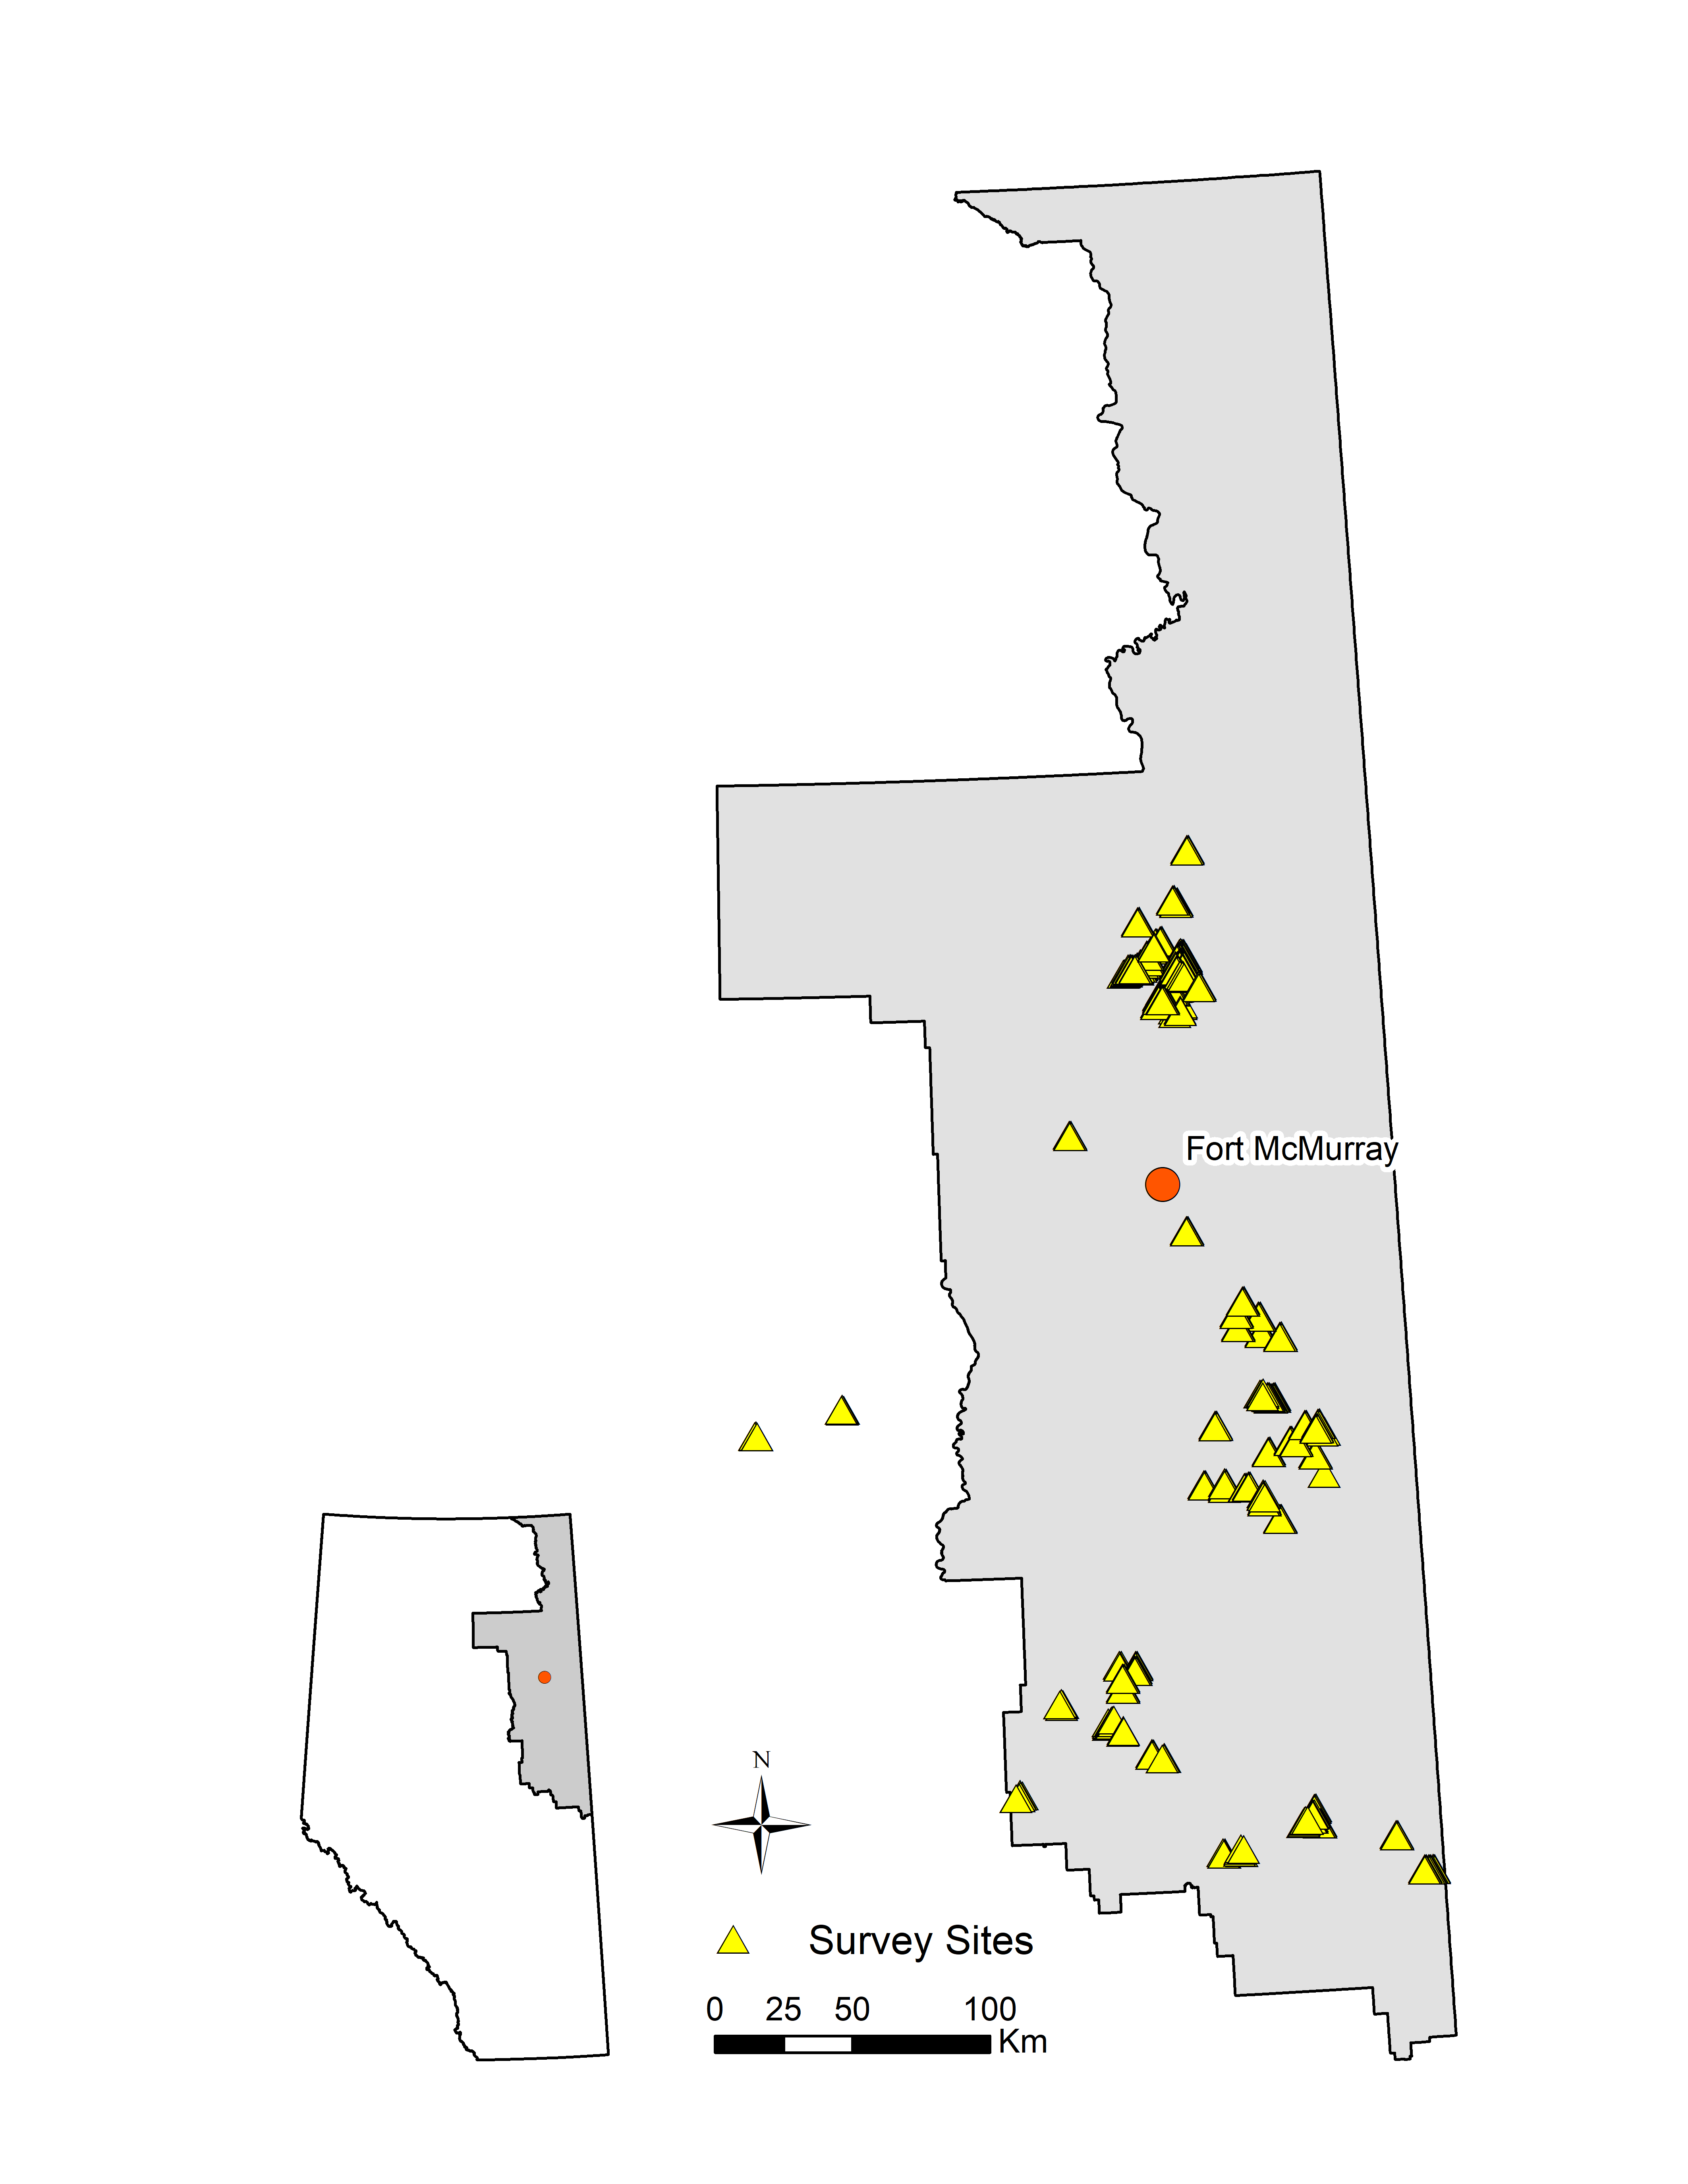
\includegraphics[width=0.75\linewidth]{C:/Users/mabec/Documents/R/OSM-Synthesis-YERA/./docs/pics/survey-sites} 

}

\caption{Yellow Rail survey sites visited between 2013-2018. The grey polygon is the Lower Athabasca planning region.}\label{fig:survey-sites}
\end{figure}

\begin{longtable}[]{@{}lrrr@{}}
\caption{\label{tab:wetlands}Regionally Important Wetlands for Yellow Rail
Breeding Habitat in the OSR.}\tabularnewline
\toprule
Wetland & Number of Monitoring Sites & Number of Males Detected &
Habitat Size (km2)\tabularnewline
\midrule
\endfirsthead
\toprule
Wetland & Number of Monitoring Sites & Number of Males Detected &
Habitat Size (km2)\tabularnewline
\midrule
\endhead
Eastern McClelland Fen Mine & 140 & 65 & 52.2\tabularnewline
Western McClelland Fen Mine & 71 & 53 & 17.3\tabularnewline
Grazing Lease 820577 & 10 & 47 & 3.4\tabularnewline
Southern Cold Lake & 15 & 30 & 4.4\tabularnewline
Marguerite Lake Wetlands & 14 & 27 & 7.4\tabularnewline
West of Touchwood PRA & 5 & 15 & 0.8\tabularnewline
Northwest of Janvier & 20 & 12 & 9.0\tabularnewline
\bottomrule
\end{longtable}

\subsection{Trend Analysis}\label{trend-analysis}

\subsubsection{Methods}\label{methods}

For this analysis we estimated a dynamic site-occupancy model (MacKenzie
et al., 2003), which allows for inference about the occurrence of Yellow
Rail at collections of sites, and about how changes in occurrence are
driven by local colonization and extinction. These models are dynamic in
the sense that they are applied to multiple ``periods'' (years, in our
case) and allow for between-period occurrence dynamics (i.e.~a rail may
be present one year, but not the next). In a monitoring context such as
ours, site occupancy probabilities can be used as a metric to reflect
the current state of the population of interest (MacKenzie et al.,
2003).

Dynamic occupancy models are also able to account for imperfect
detection probability (i.e., a rail can go unobserved at a site during a
particular survey, even if it is there). An occupancy model may be
seriously biased if detection error is unaccounted for (Moilanen, 2002;
Royle and Dorazio, 2008). This bias is manifested as underestimates of
site occupancy and inflated estimates of species turnover rate, where
apparent recolonization of a site is actually just due to non-detection
of a species actually present.

We use the package \texttt{unmarked} (Kery and Chandler, 2016) to fit a
dynamic occupancy model to our Yellow Rail data using the function
\texttt{colext()} in R v3.6.1 (R Core Team, 2019). To better understand
variation within the region, we subset our data into four geographic
areas and occupancy analysis is conducted on each: the Eastern
McClelland Fen Mine (n = 140), Western McCelland Fen Mine (71), all
Mineable Areas (226), and Non-Mineable Areas (269). The analysis is
conducted using all sites together as well (Full Region).

\subsubsection{Detection, Colonization, and
Extinction}\label{detection-colonization-and-extinction}

Detection is the proportion of visits to a site where a species is
detected. Rather than using this straight proportion, this model
accounts for imperfect detection probability using the method described
in MacKenzie et al (2003).

Detection probability by regional subset is displayed in Figure
\ref{fig:detection-comb} below, followed by the full region (Figure
\ref{fig:detection-full}. The error bars represent 90\% confidence
intervals in the estimated detection parameter.

\begin{center}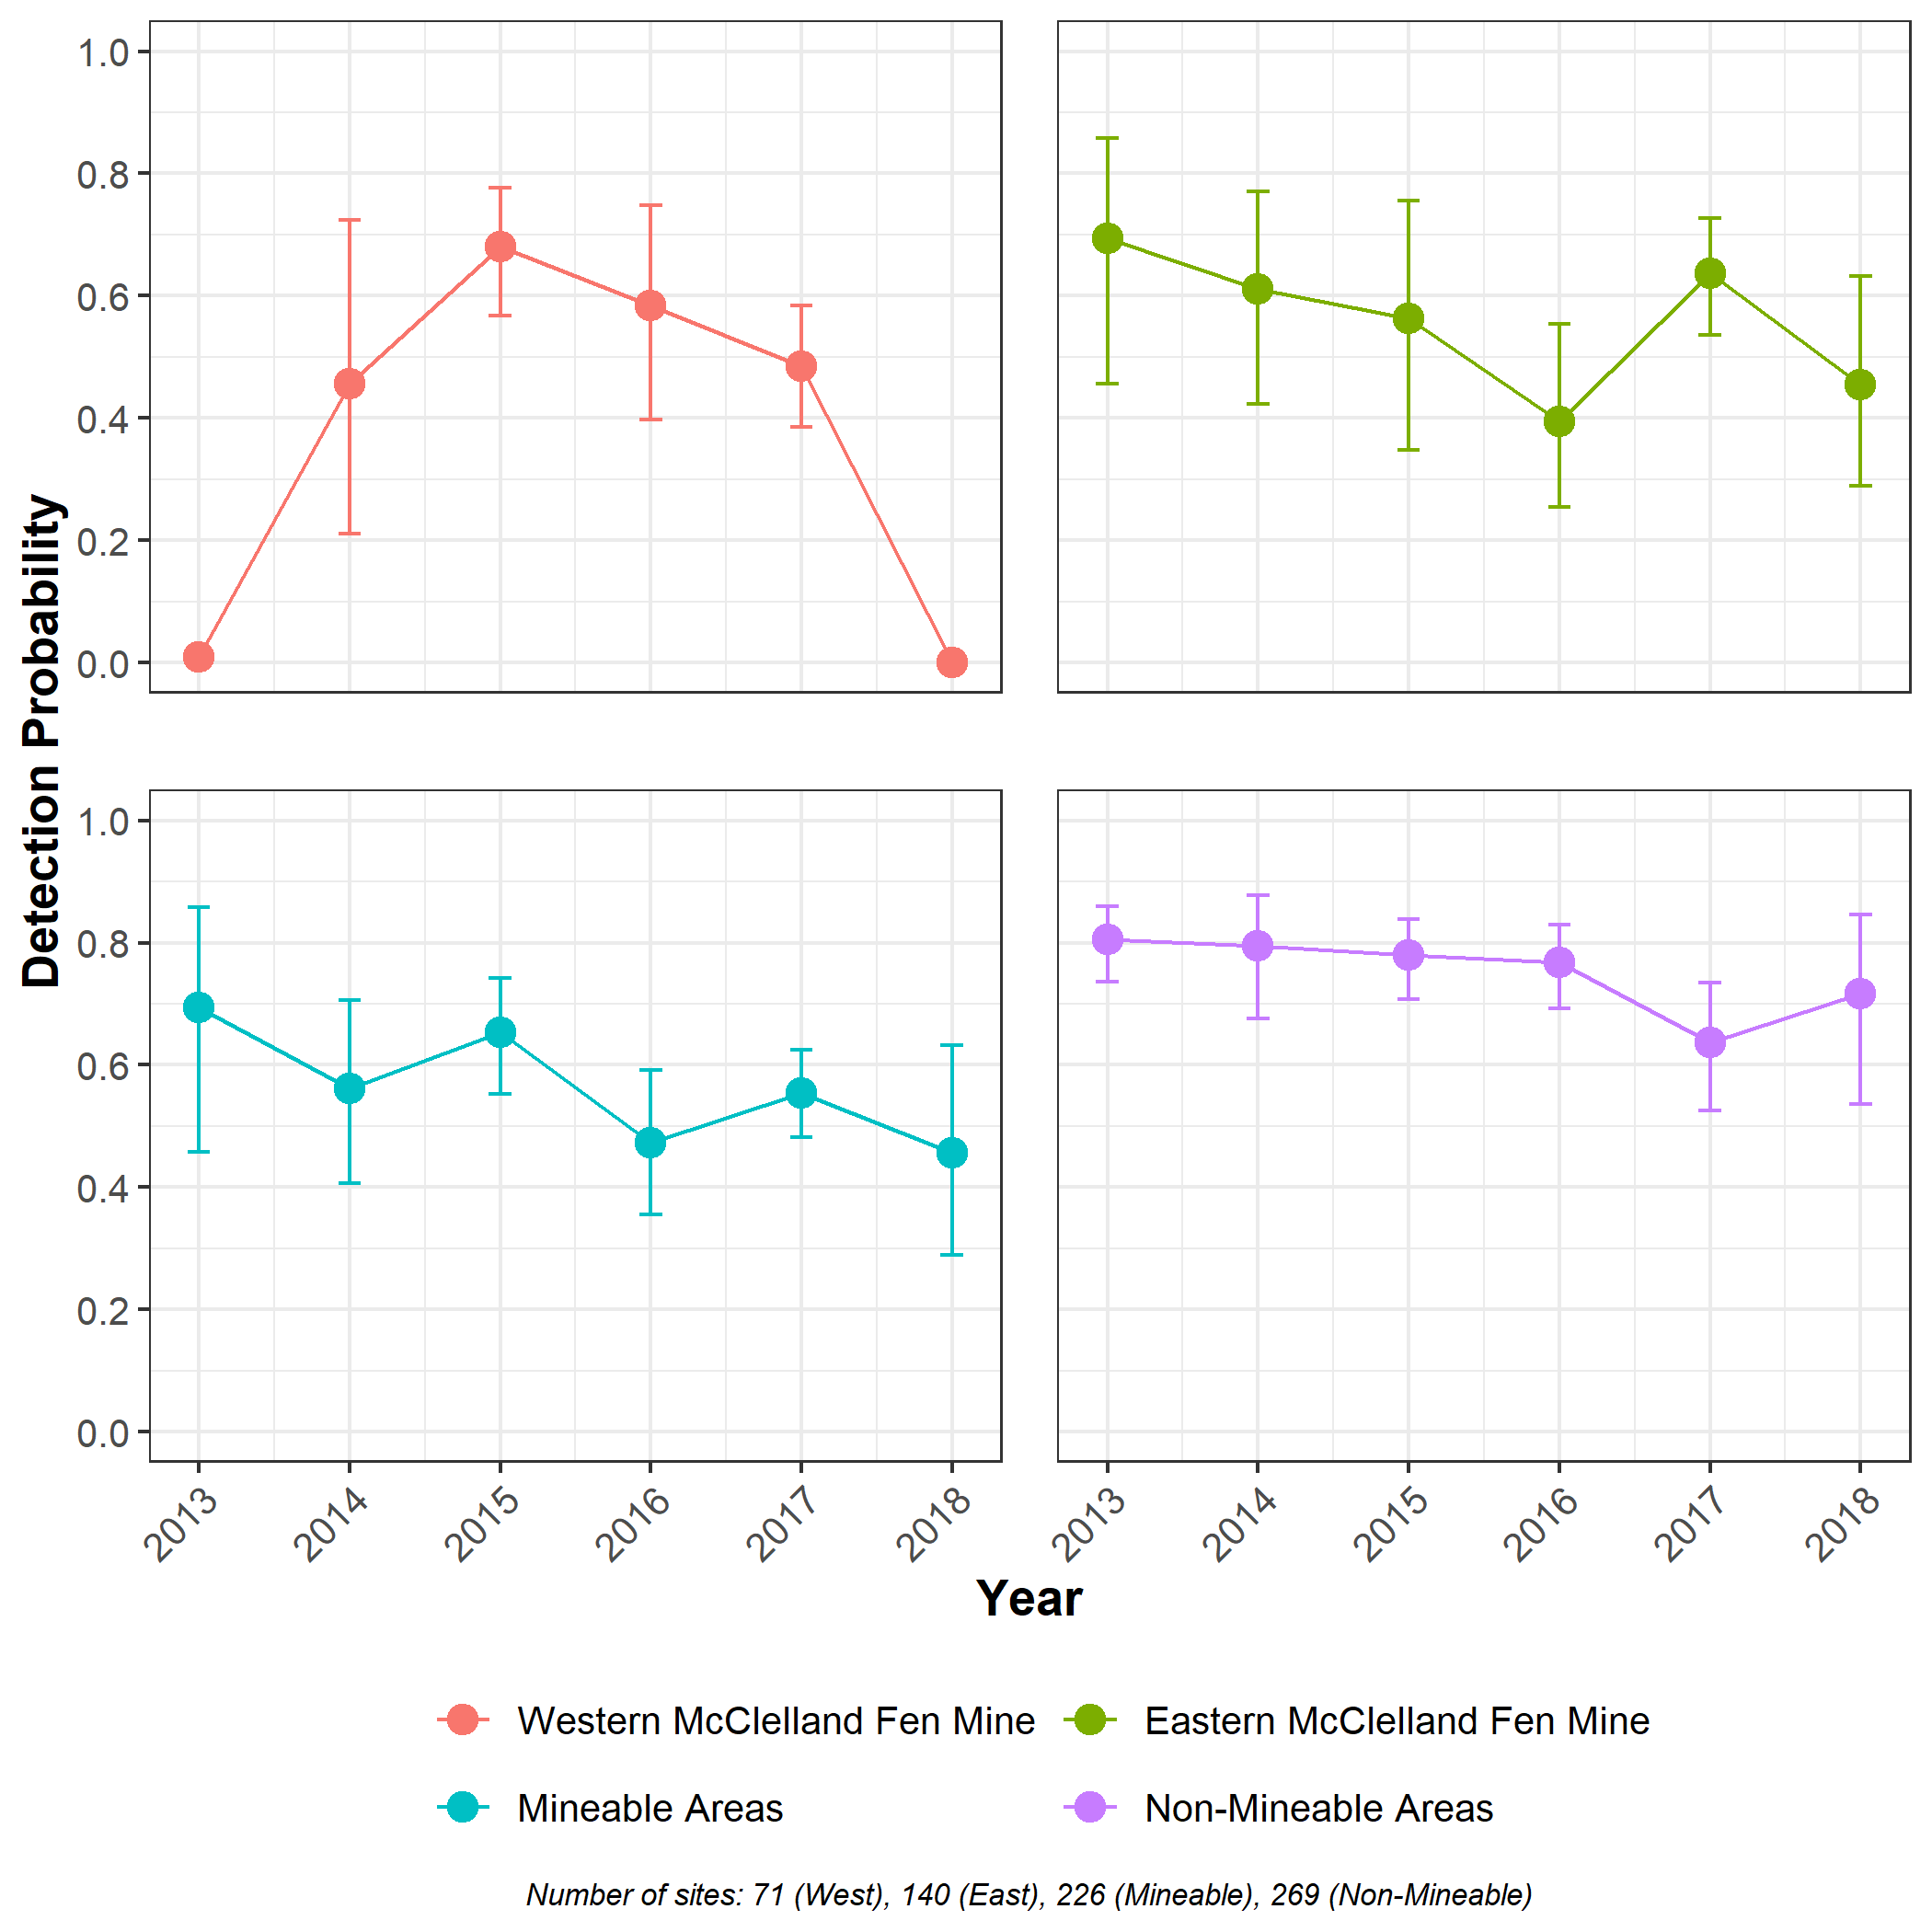
\includegraphics[width=1\linewidth]{C:/Users/mabec/Documents/R/OSM-Synthesis-YERA/./docs/pics/detection-comb} \end{center}

\begin{center}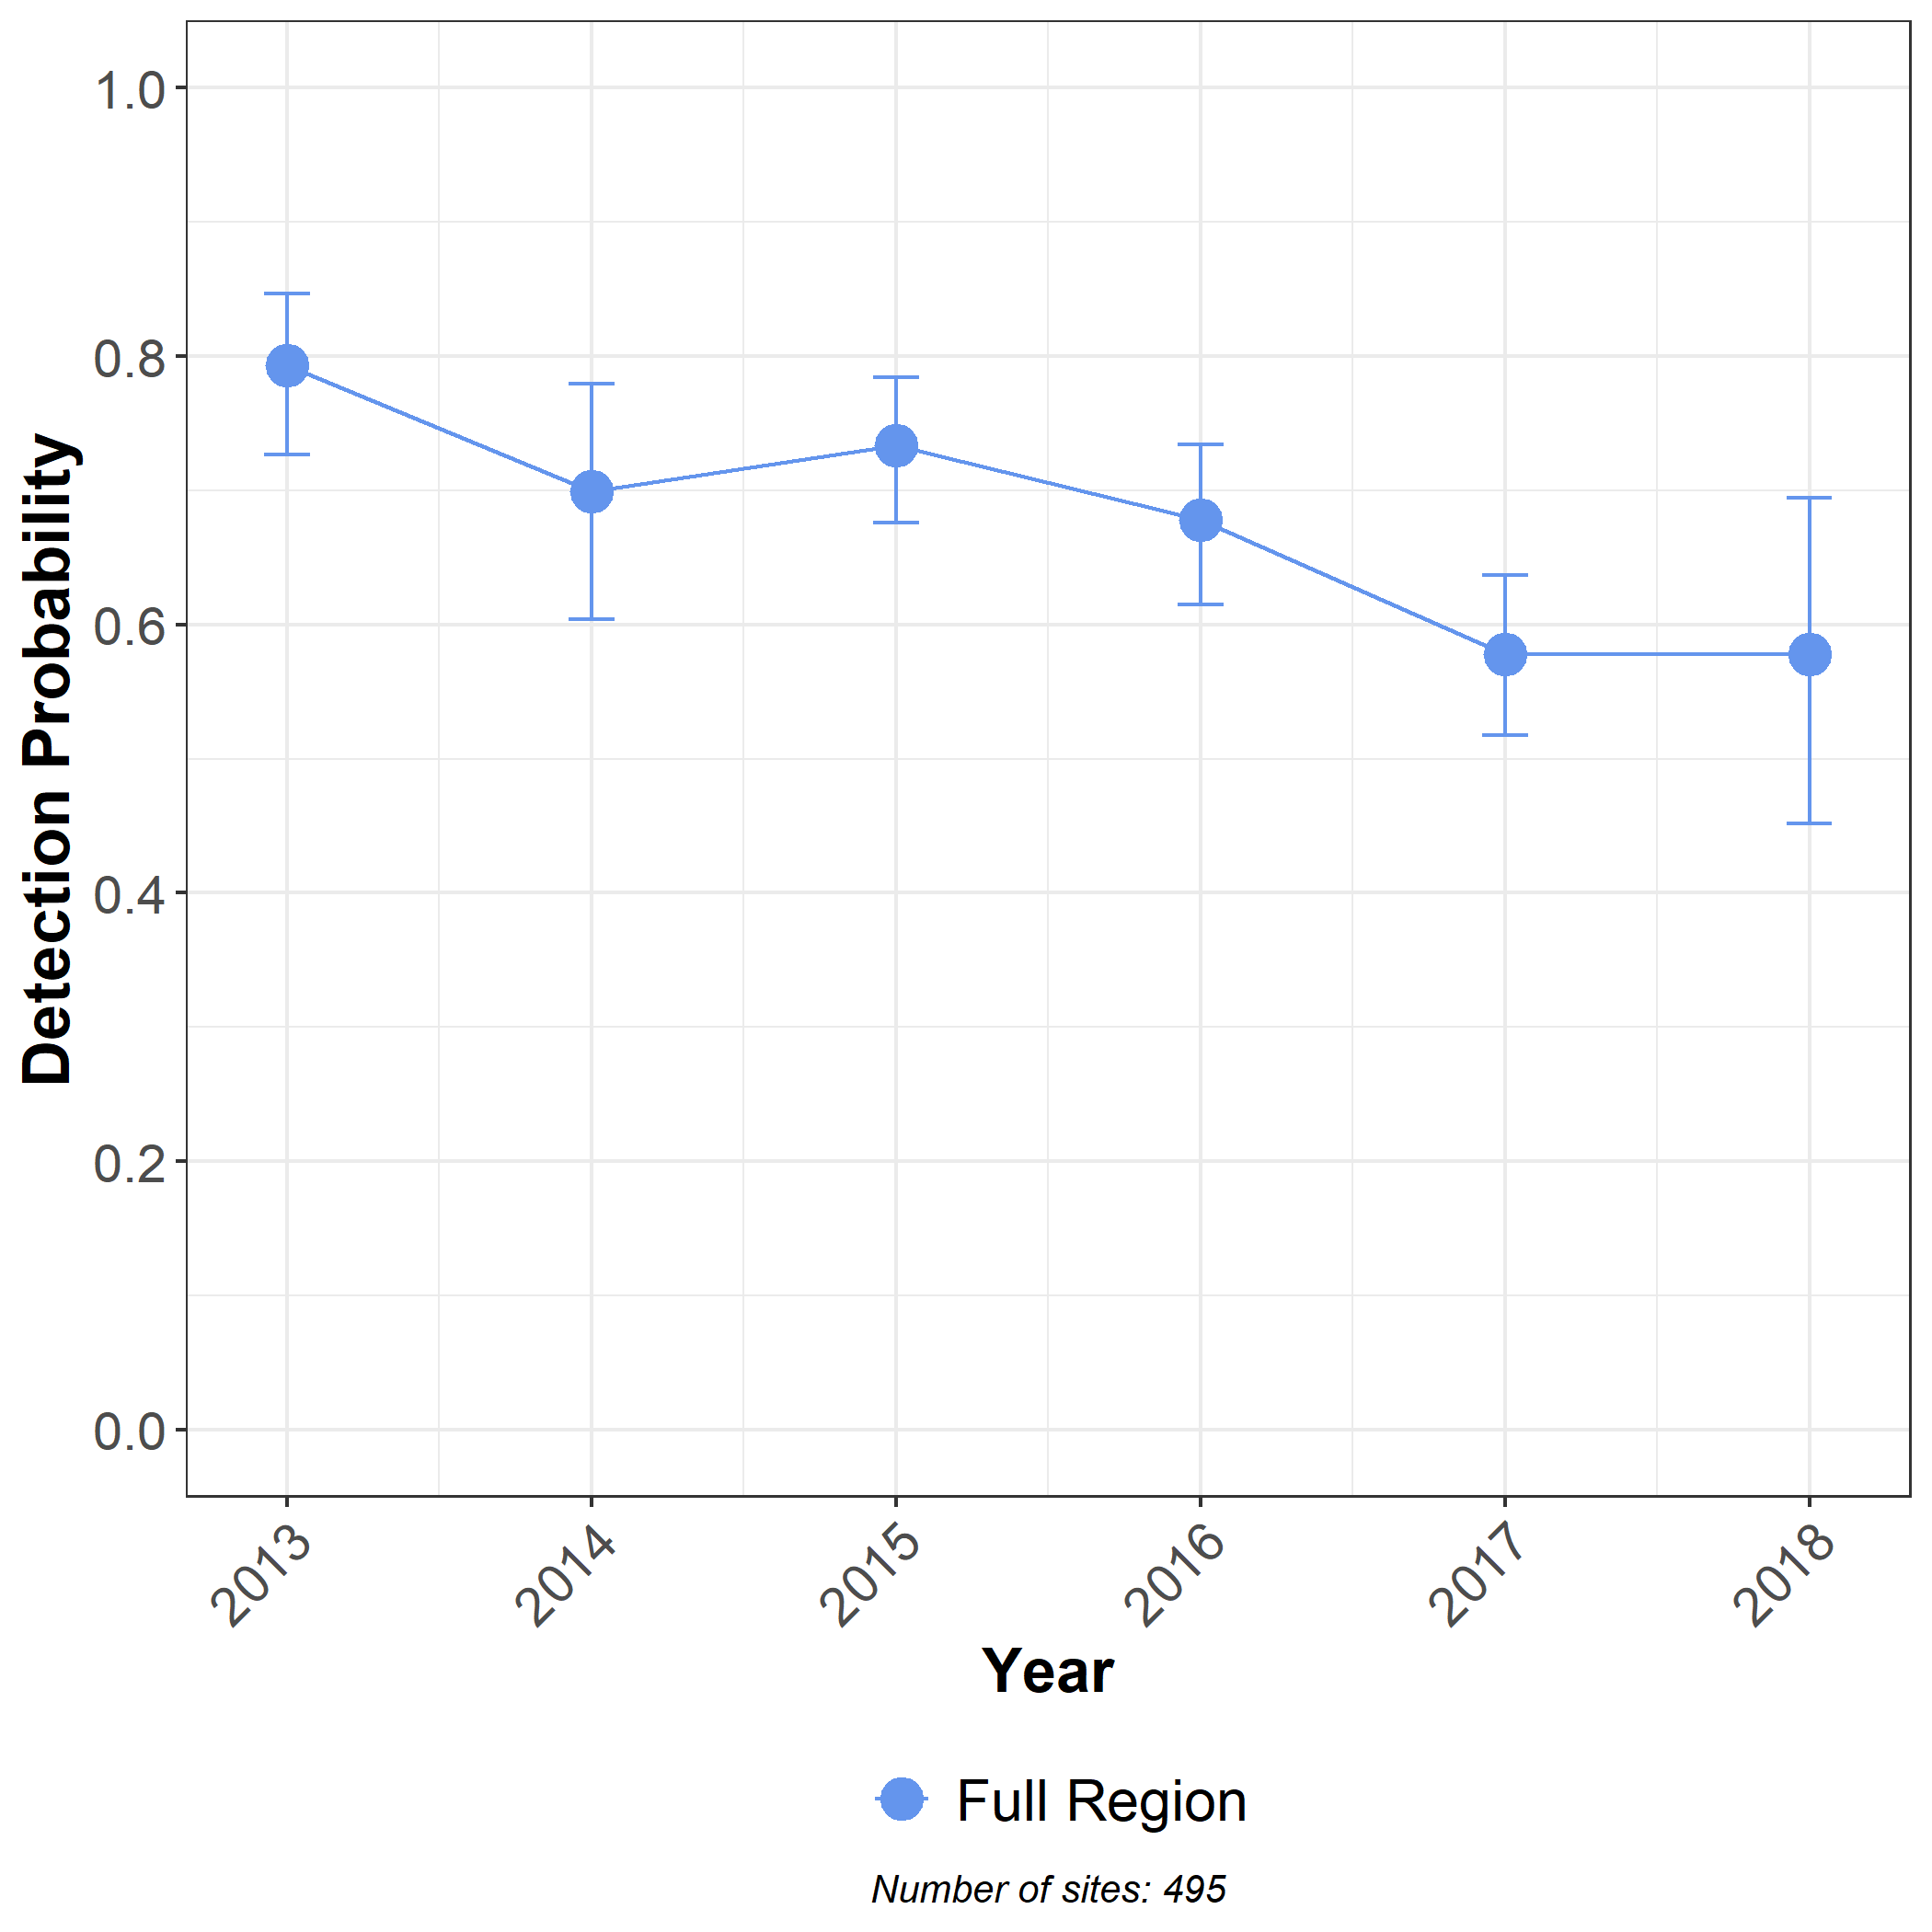
\includegraphics[width=0.7\linewidth]{C:/Users/mabec/Documents/R/OSM-Synthesis-YERA/./docs/pics/detection-full} \end{center}

Detection probability can be influenced by a variety of factors. First,
individuals may call less in a given year for unknown reasons. This
could lead to lower detection rates but stable occupancy. Alternatively,
detection rates increase when there are more individuals present at a
location (Bayne et al. 2017). Thus, the decline we see in detection
rates may reflect the species still occupying the same number of sites
but fewer individuals being present at some sites leading to lower
detection rates (i.e.~the same number of sites are occupied but fewer
individuals are present at each site). We are currently working on
analyses that use the count of yellow rails at each site.

Changes in occurrence of a species can be driven by rates of both
colonization and extinction at a set of local sites. Colonization is
probability that an unoccupied site becomes occupied in the next period;
conversely, extinction (or alternatively, survival) describes the
probability that an occupied site continues to be occupied in the next
period.

Predicted colonization and extinction parameters are displayed below for
each regional subset (Figure \ref{fig:extinction-colonization-comb}),
followed by the two parameters for a full regional model (Figure
\ref{fig:extinction-colonization-full}). Error bars represent a 90\%
confidence interval in the estimated colonization and extinction
parameters.

\begin{center}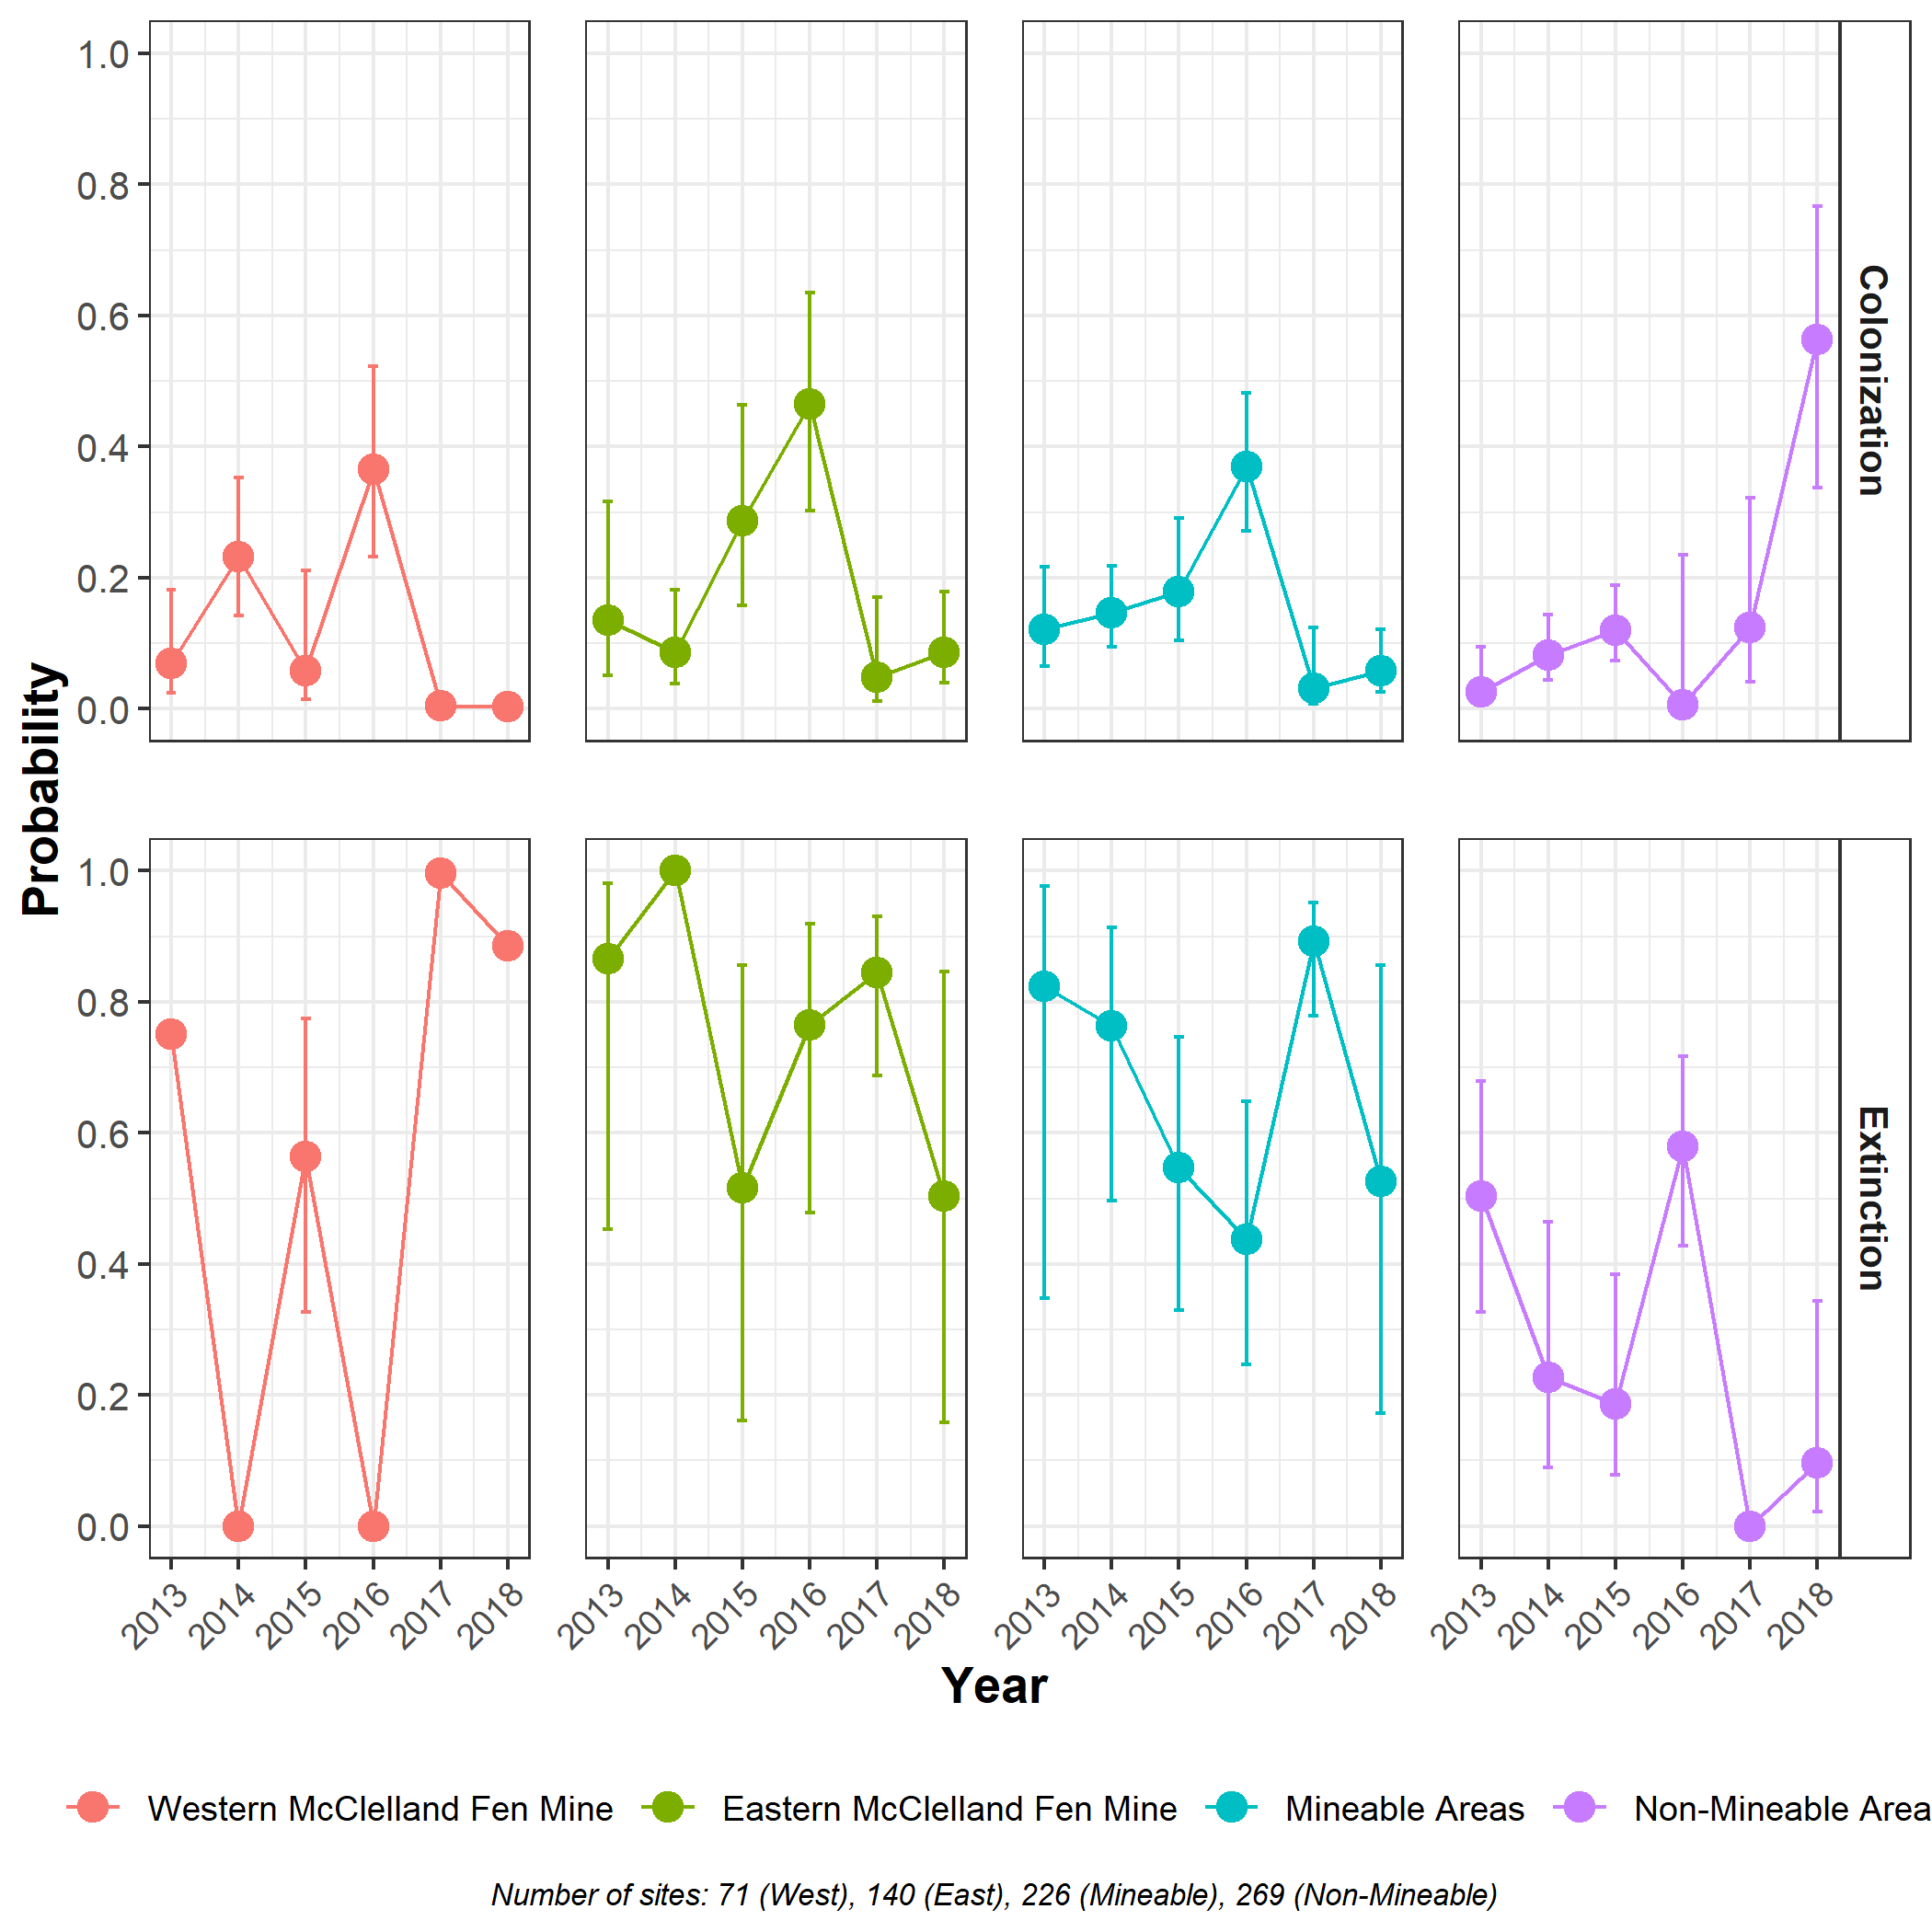
\includegraphics[width=1\linewidth]{C:/Users/mabec/Documents/R/OSM-Synthesis-YERA/./docs/pics/extinction-colonization-comb} \end{center}

\begin{center}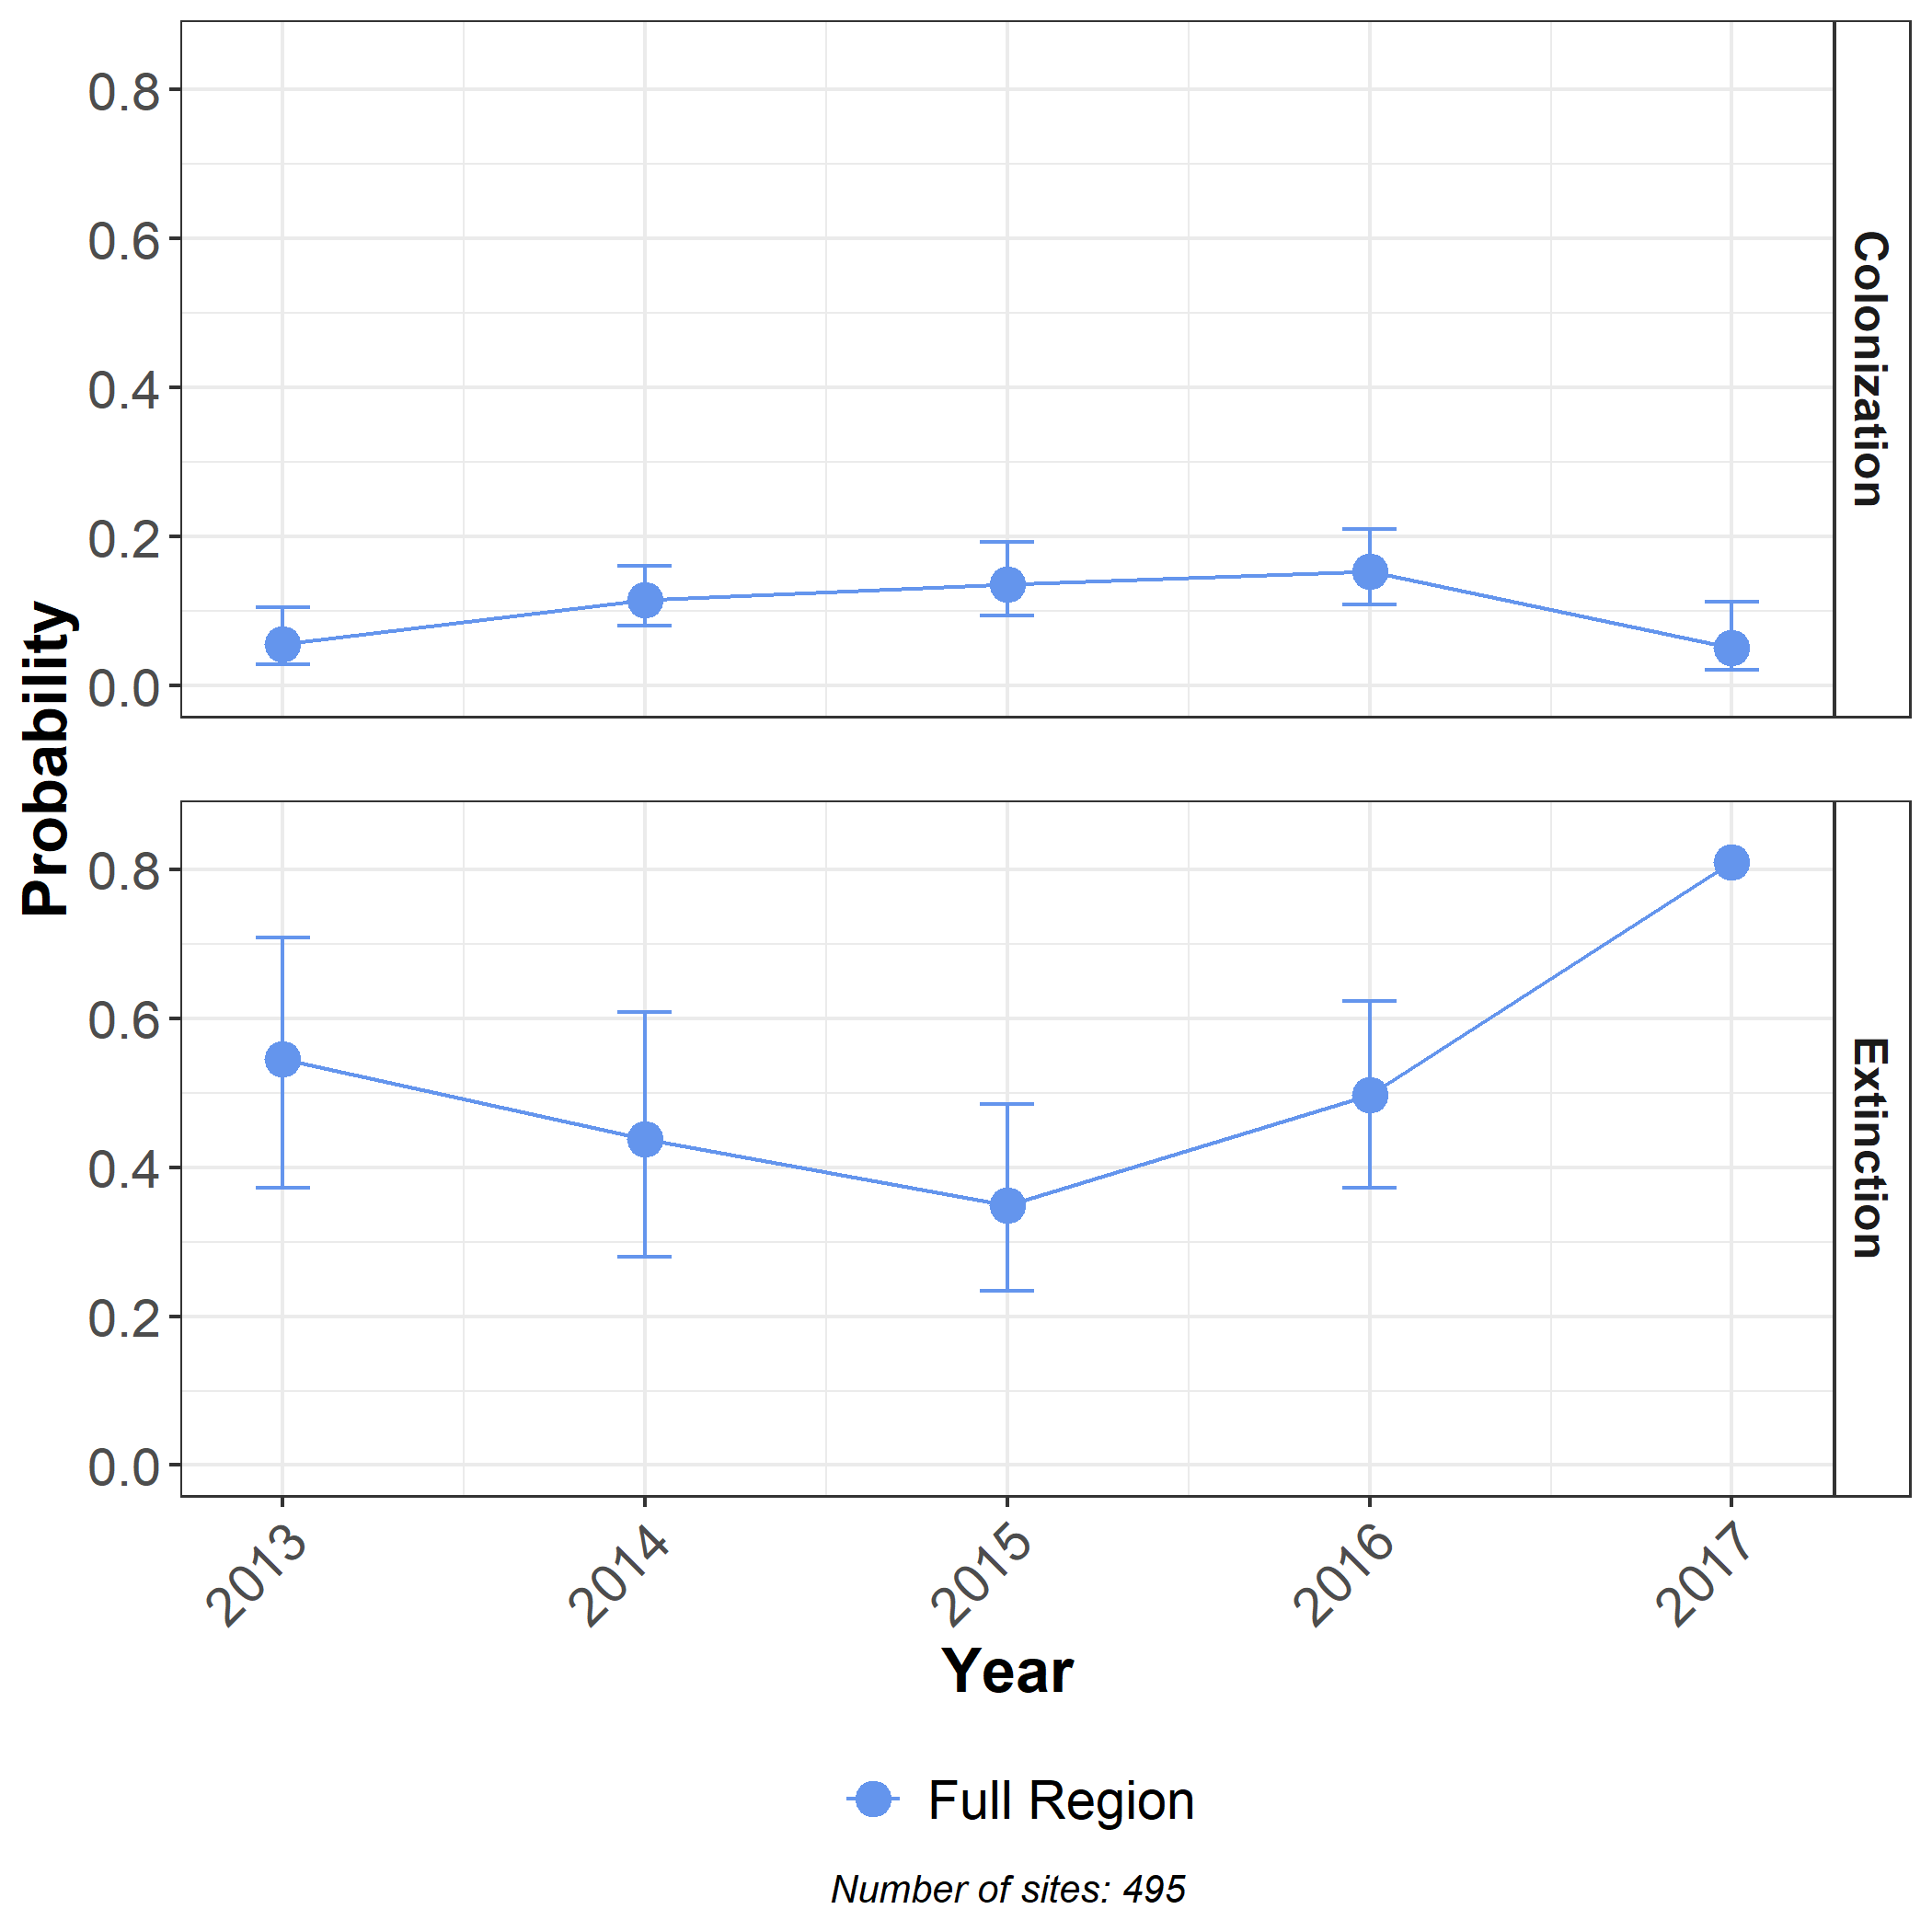
\includegraphics[width=0.7\linewidth]{C:/Users/mabec/Documents/R/OSM-Synthesis-YERA/./docs/pics/extinction-colonization-full} \end{center}

The high rates of extinction and colonization show that the local
dynamics of the Yellow Rail are highly variable over time. Thus, any
short-term disappearance from a site (i.e.~the Western McLelland fen) is
not neccesarilly cause for concern as there is reasonable probability
that they will recolonize the area when water levels are appropriate
(see occupancy discussion below).

\subsubsection{Occupancy}\label{occupancy}

Occupancy, adjusted for imperfect detection, is estimated for each of
the four regional subsets between 2013 and 2018, and the results are
displayed in Figure \ref{fig:occ-comb}. Occupancy is also estimated for
the full region and displayed in Figure \ref{fig:occ-full}.

\begin{center}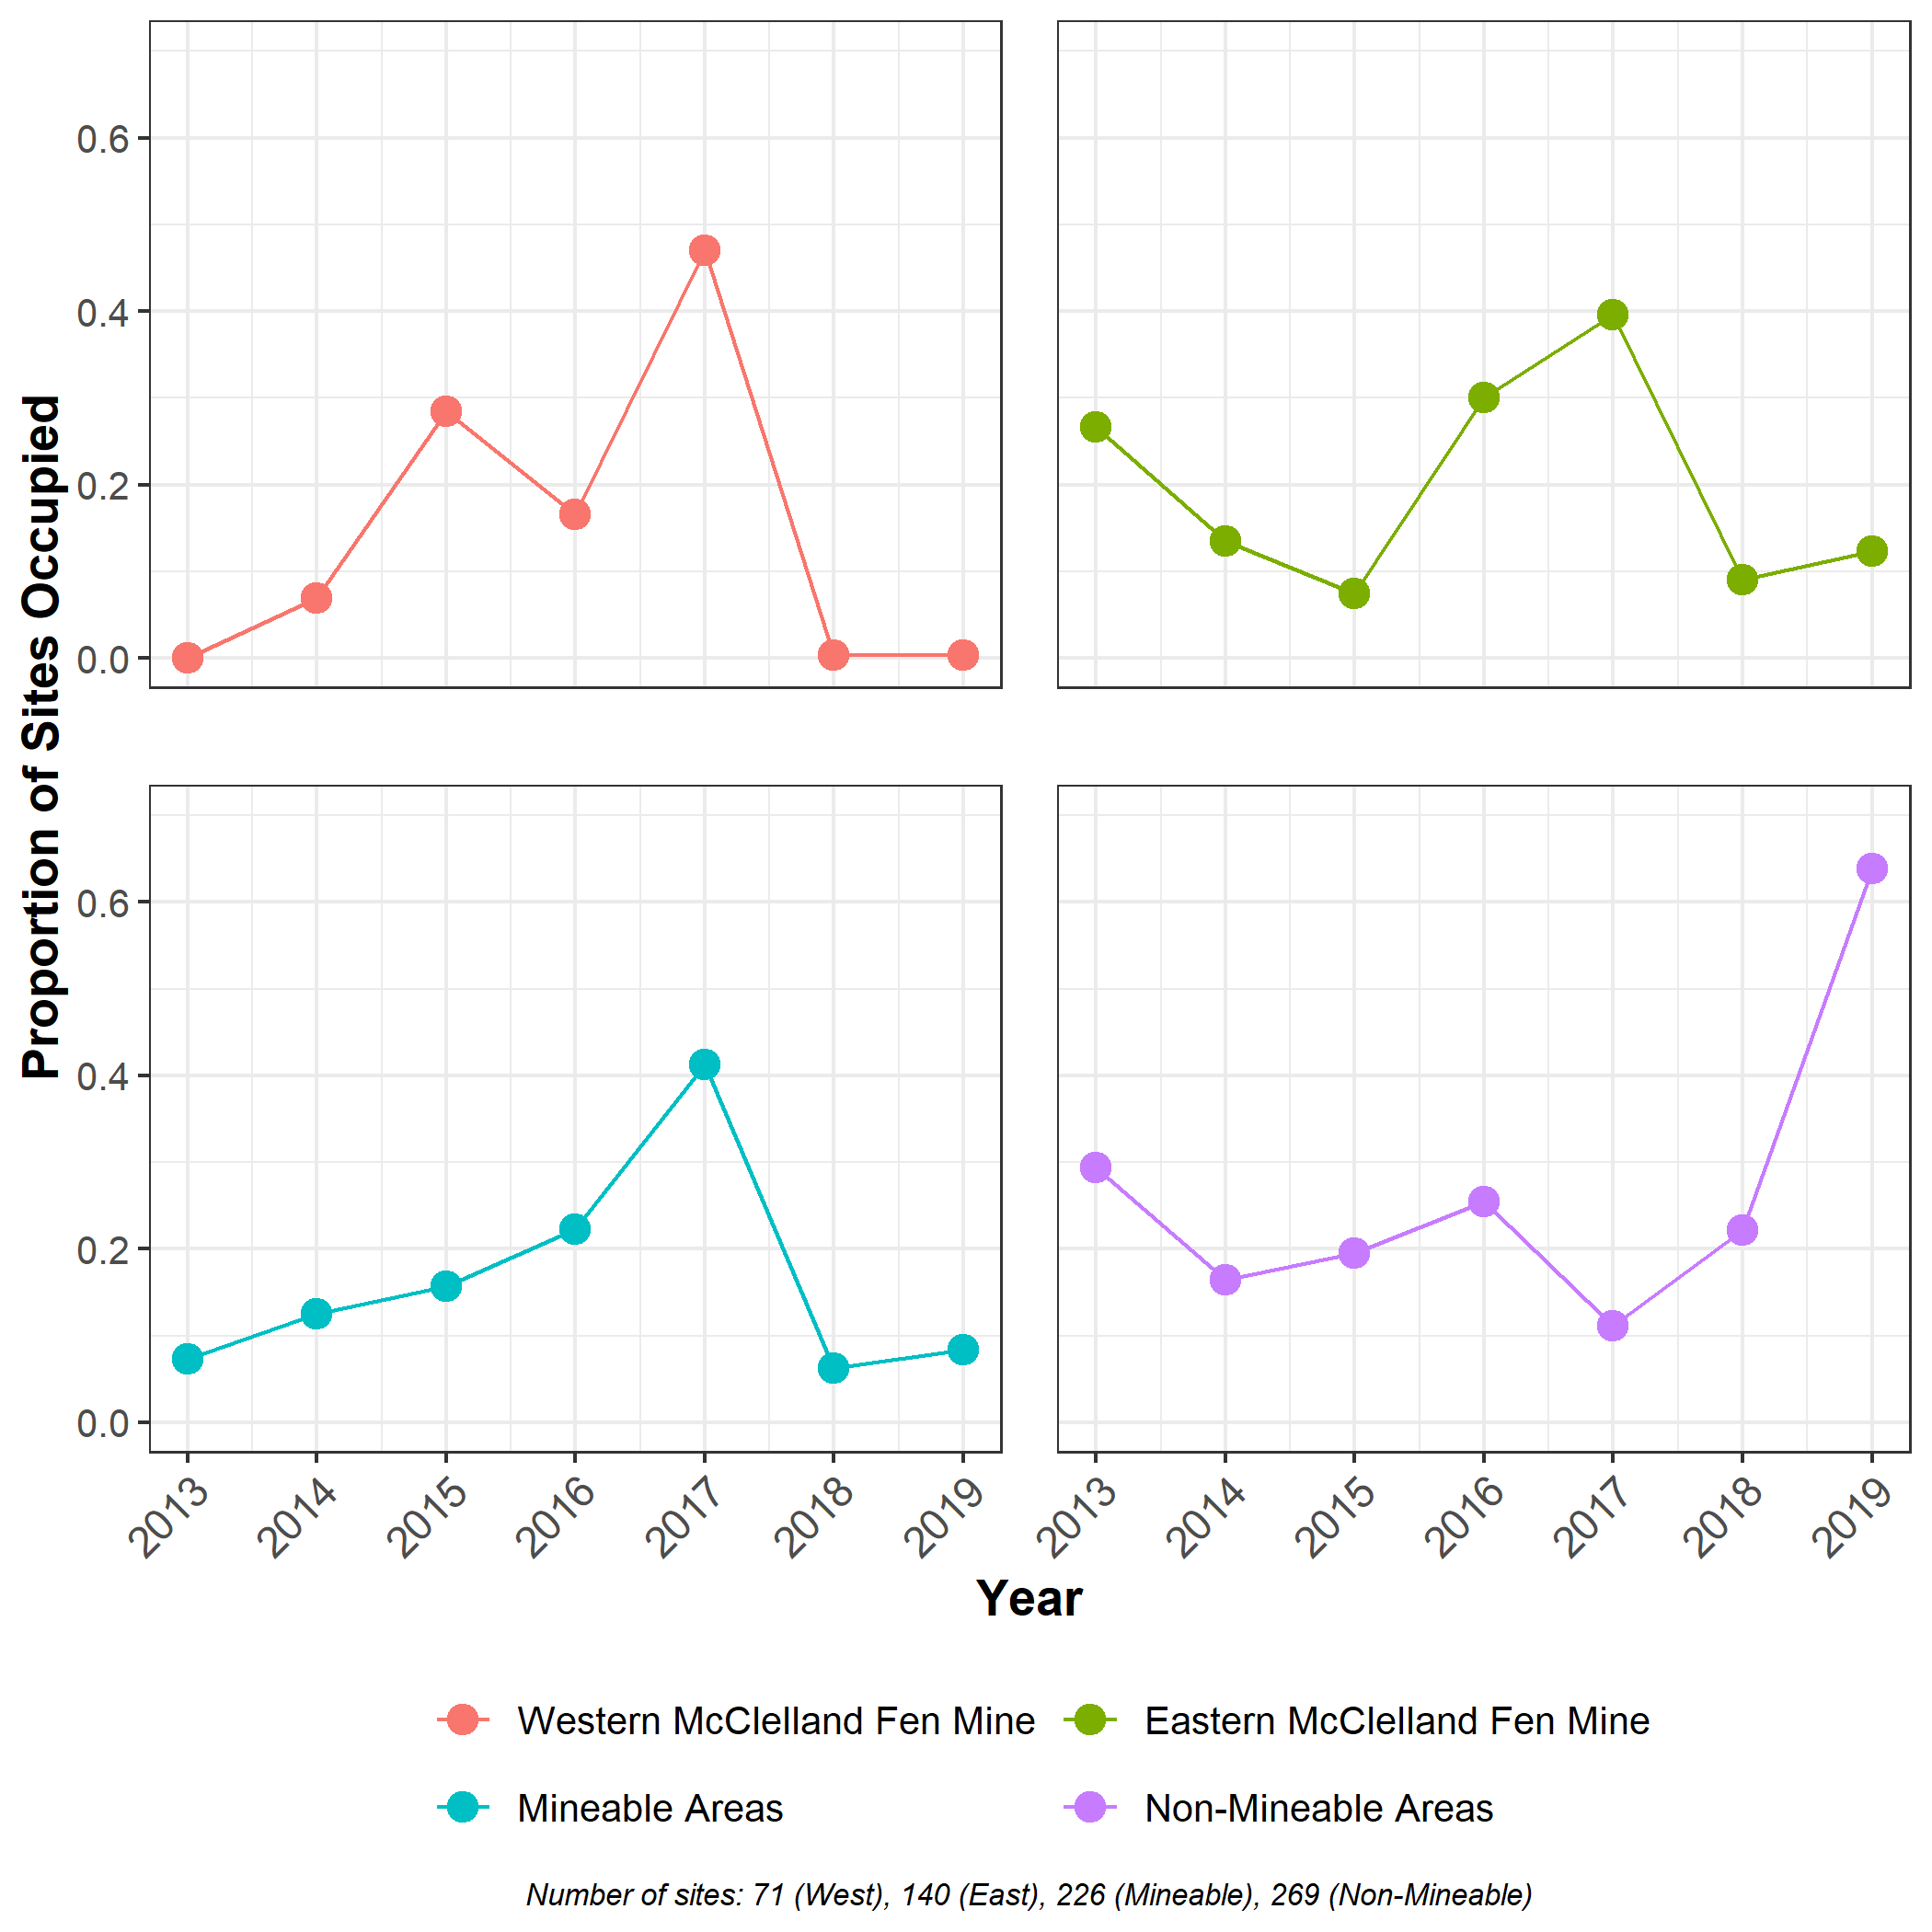
\includegraphics[width=0.85\linewidth]{C:/Users/mabec/Documents/R/OSM-Synthesis-YERA/./docs/pics/occ-comb} \end{center}

Occupancy is also estimated for the full region, including all sites.

\begin{center}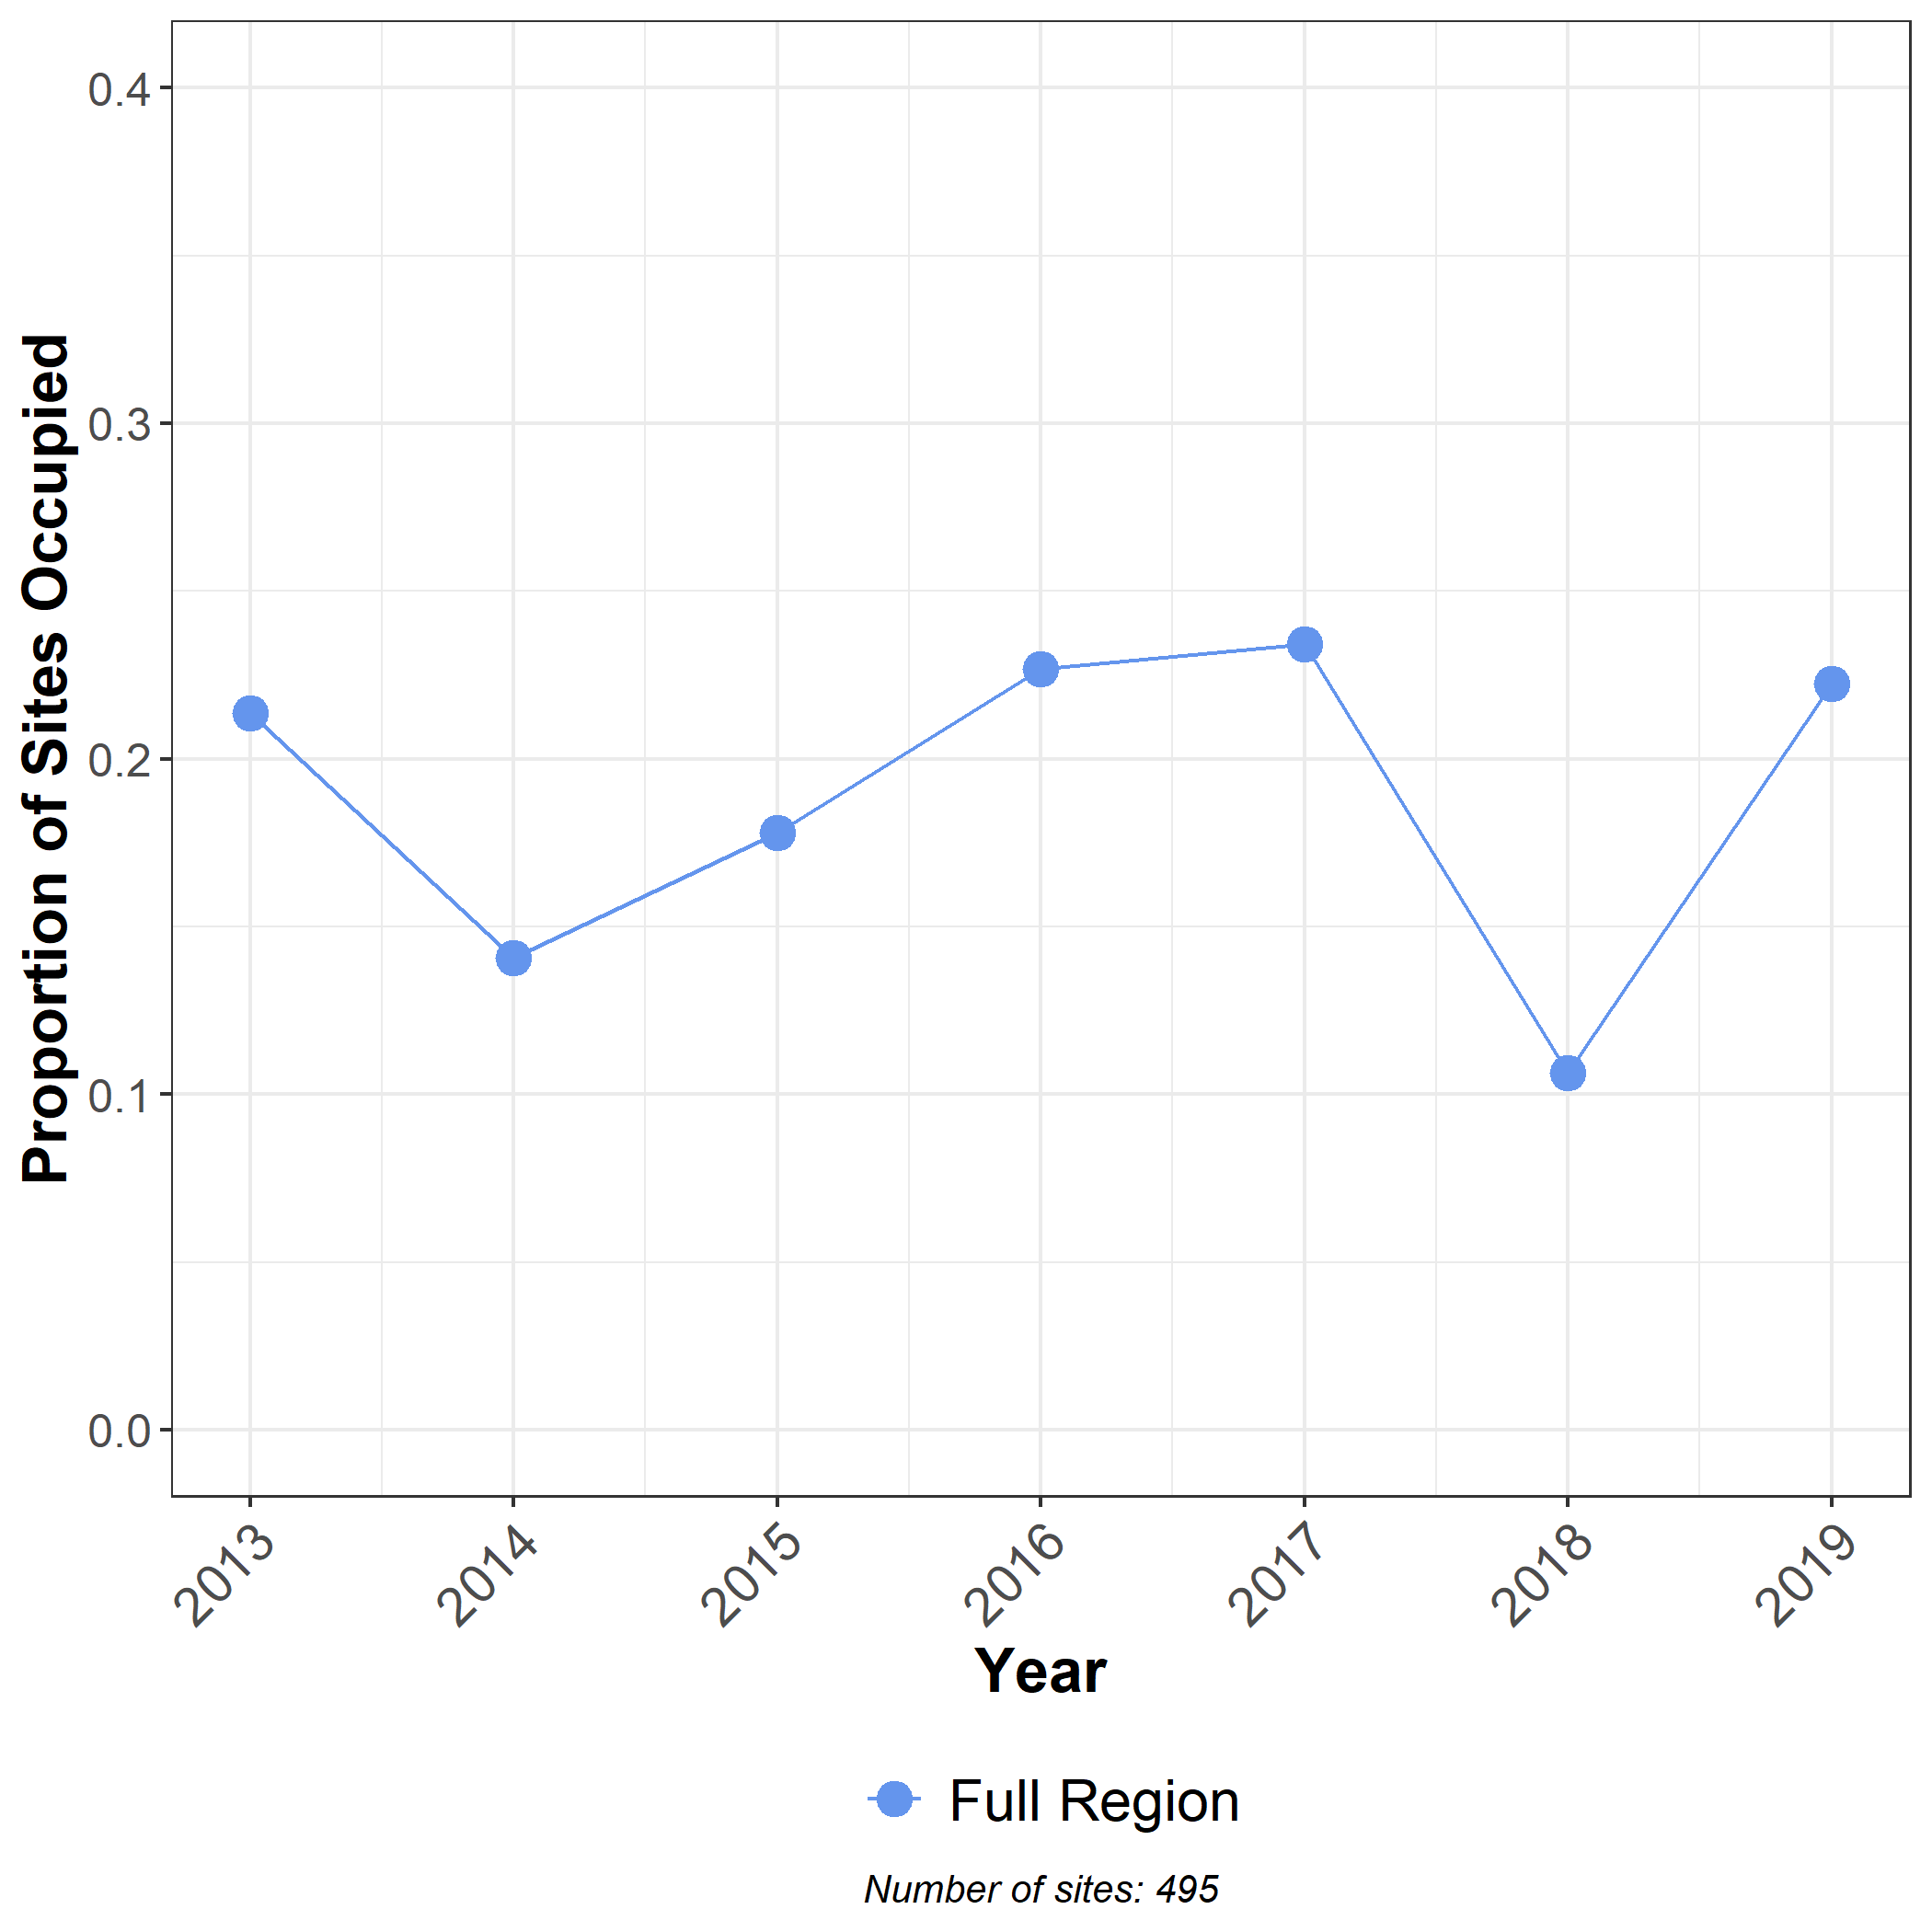
\includegraphics[width=0.7\linewidth]{C:/Users/mabec/Documents/R/OSM-Synthesis-YERA/./docs/pics/occ-full} \end{center}

One aspect of the data worth noting is the drop in occupancy rates in
2018 in the Western McLelland fen. Occupancy rates were approximately
0.45 in 2017, and dropped to 0 in 2018. This may be a cause for concern
from a conservation perspective, as this section of wetland is adjacent
to ongoing developments (Suncor Fort Hills mine). However, a causal link
cannot yet be drawn for a few reasons. First, consistent with the
existing literature on this species, Yellow Rail occupancy fluctuates
greatly year-to-year in individual wetlands. Linking changes in
occupancy to causal mechanisms is complicated by the inherent noisiness
of the data. Second, the potential decline occurred only in the most
recent year; until 2018, the number of occupied Yellow Rail sites had
been consistently increasing in the Mineable region. Additional years of
data would be helpful to assess whether this represents a change in
habitat suitability or simply natural fluctuations. In fact, data from
2013 also showed low occupancy rates in the western fen, suggesting 2018
may not have been anomalous. Data from 2019 have been collected and will
help answer these questions, but monitoring in 2020 and beyond will
likely be needed to draw strong conclusions.

\subsubsection{Further Analysis}\label{further-analysis}

To better understand the between-year dynamics of Yellow Rail occupancy,
certain environmental conditions or attributes of each site could be
added as covariates to the occupancy model. Evidence suggests that
Yellow Rail are sensitive to changes in water levels, and even modest
changes in hydrology may render habitat unsuitable as a breeding site
(Austin and Buhl, 2013; COSEWIC, 2009). Where oil sands development (or
potential development) encrouches upon Rail habitat (such as around
McClelland Lake), changes to hydrology may pose as big a threat as
direct habitat removal. Adding measurements of water depth levels taken
during field sampling to the occupancy model may help explain variation
in occupancy rates both between years and between sites. Since 2013,
water depth levels have been recored at 0, 10, 20, 30, 40 and 50-m
intervals in four directions (SE, SW, NE, and NW) from each monitoring
site.

Preliminary work has been done to include water measurements in a model
of Yellow Rail occupancy, which will be presented in an updated version
of this report. Below is displayed boxplots of the distribution in
predicted water depth for each year and for three regions of interest:
the Eastern McClelland Fen Mine, Western McClelland Fen Mine
(\ref{fig:water-depth-mcclelland}), and unmineable sites
(\ref{fig:water-depth-unmineable})\footnote{Note that this regional
  population estimate applies to the area covered by the habitat
  suitability map, not the OSR as a whole.}. A mixed effect model was
used, with the log transform of water depth at the response, year and
date as independent variables, and monitoring site as a random effect. A
Poisson link function was used.

\begin{figure}[H]

{\centering 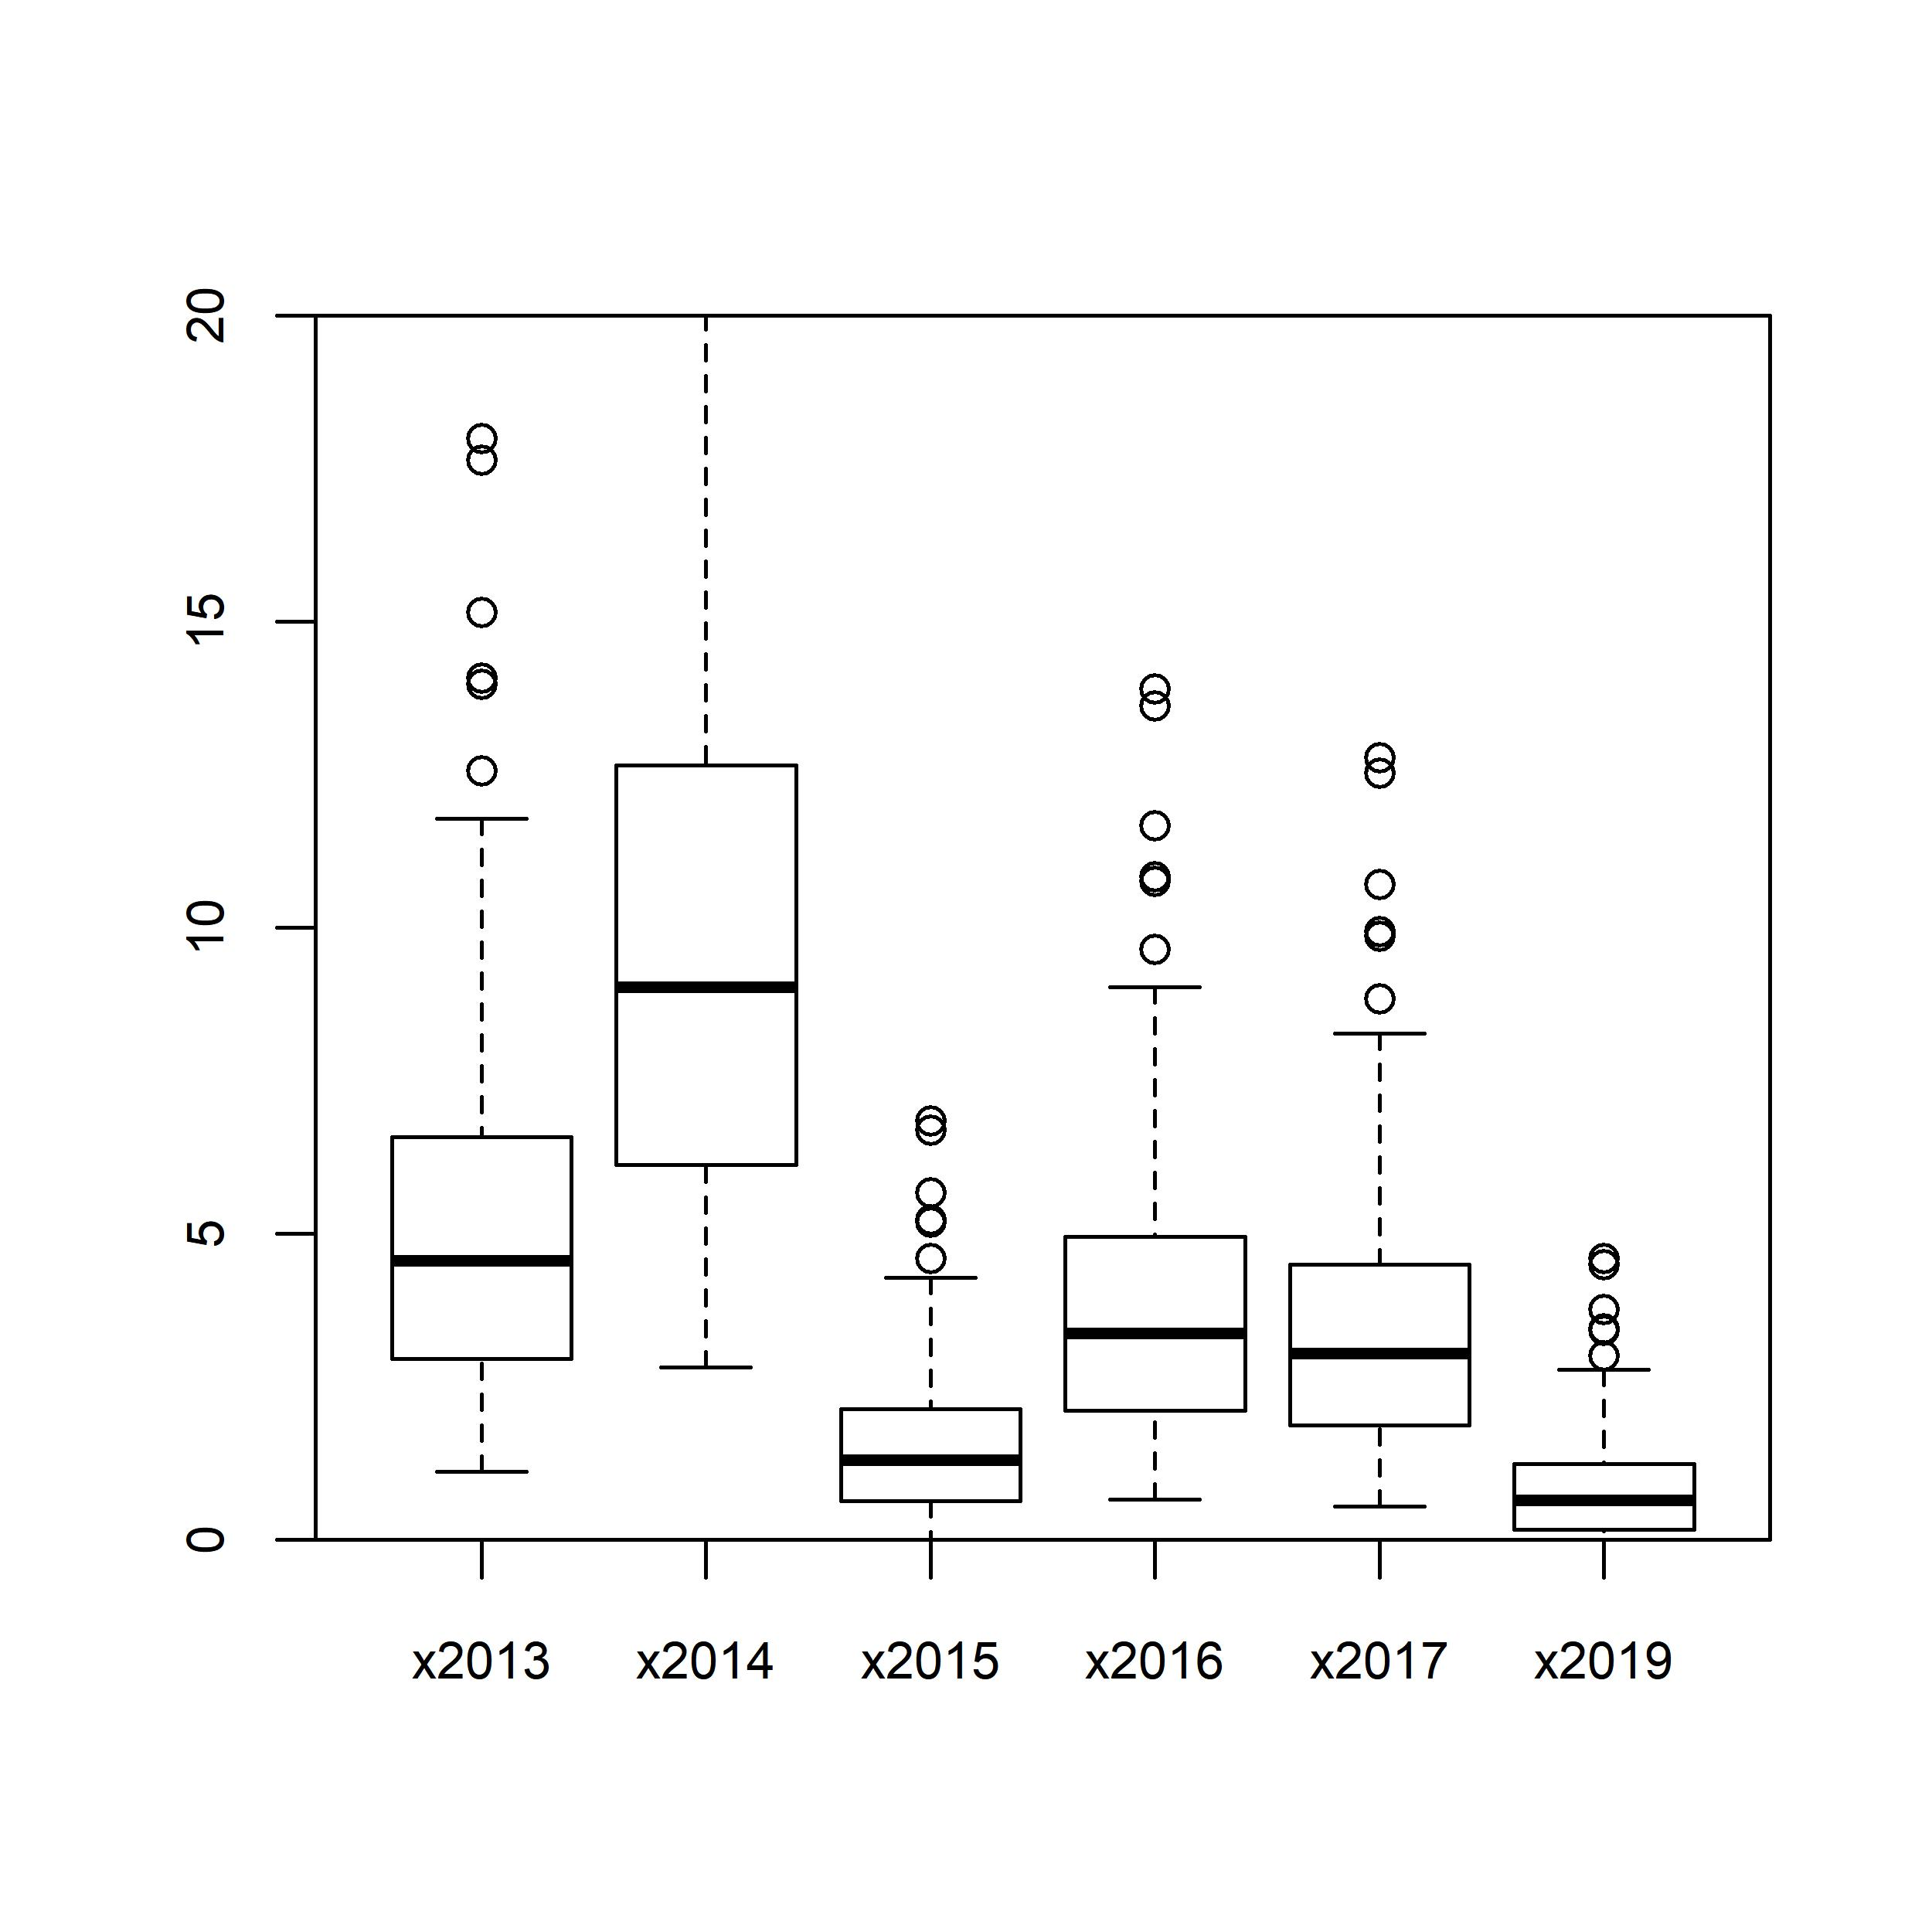
\includegraphics[width=0.5\linewidth]{C:/Users/mabec/Documents/R/OSM-Synthesis-YERA/./results/unmineableWaterDepthByYear} 

}

\caption{Water depth in the unmineable region.}\label{fig:water-depth-unmineable}
\end{figure}

Distance to mine edge has also been hypothesized as an important
predictor of Yellow Rail occupancy at surveyed sites. The map below
outlines how mine footprint (ABMI, 2017) has changed near McClelland
Lake (both west and east portions of the fen) throughout the study
period, along with variation in site occupancy. Mine encrouchment does
not appear to alter spatial patterns of rail occupancy, as detections
are found both close to and far from mine edges. However, further work
will be required to test this effect.

\subsection{Threats to Known Breeding
Sites}\label{threats-to-known-breeding-sites}

Several oil sands leases overlap with important breeding sites for
Yellow Rails in the OSR, most notably the west and east areas of the
McLelland Lake Fen. This interconnected fen complex contains a vast area
of suitable habitat and large numbers of breeding individuals each year.
The reader can view this overlap in the above map through the `Nearby
Oil Sands Lease Sites' layer.

The western portion of the McClelland Lake Fen is overlapped by the Fort
Hills Oil Sands Project lease. About 55\% of the identified suitable
habitat in the area lies within the lease, a portion which includes 66\%
(35 of 53) of the Yellow Rails detected in the western McClelland Lake
Fen since 2012.

A number of developments, or proposed developments, overlap with Yellow
Rail habitat on the eastern portion of the McClelland Lake fen as well.
Rails have been detected in the proposed footprint of both the Jackpine
Mine Phase 2 and Kearl Oil Sands Projects (30\% of individuals detected
in the area since 2012). Yellow Rails were also detected in Aurora Mine
South, and although no detections have been recorded recently, past
surveys have recored Rails in the Muskeg River Mine Project lease area
(Hatfield Consultants, 2008). The next section discusses the potential
Yellow Rail habitat in each lease area, much of which has yet to be
surveyed.

\section{Planning Tools}\label{planning-tools}

\subsection{Habitat Suitability Map}\label{habitat-suitability-map}

Results from Yellow Rail site surveys between 2012-2017 were used to
produce a map of preferred habitat across a subset of the OSR. Four
mapping products were used to build this final `fusion' model:

\begin{itemize}
\tightlist
\item
  Alberta Biodiversity Monitoring Institute (ABMI) 2010 Landcover
  Classification. This product is an Alberta-wide (`wall-to-wall')
  provincial land cover based on digital classification of Landsat
  satellite imagery and enhanced using GIS datasets obtained from the
  Government of Alberta. It consists of 15 classes, including water,
  shrubland, grassland, agriculture, exposed land, developed land, and
  various forest types.
\item
  Ducks Unlimited Enhanced Wetland Classification. This is a western
  boreal product based on a combination of Landsat and Radarsat. Using
  object-based supervised classification methods this product identifies
  19 boreal plans wetland classes and 10 other land cover classes.
\item
  Landcover Classification of Canada. Based on MODIS satellite
  observations from 2005, the product identifies 39 classes of
  landcover.
\item
  Alberta Vegetation Inventory. AVI is a photo-based digital inventory
  developed to identify the type, extent and conditions of vegetation.
  Human observers digitize polygons into a series of forest type classes
  that include various non-forested categories. Environment and Climate
  Change Canada (Edmonton) created a classification system from the AVI
  that converted the underlying attributes into 37 unique classes of
  which nine represent wetland types.
\end{itemize}

Each of the four products were either available in, or converted to, a
30-m raster. We used a resource selection function approach based on the
logistic discriminant approach (Manly et al. 2002) to determine whether
each land-cover class within four distinct mapping products was avoided,
neutral, or selected. A land-cover class that was avoided had a beta
coefficient that was negative and a 95\% confidence interval that did
not include zero. A land-cover class that had a beta coefficient that
was positive and 95\% confidence interval that did not include zero was
selected. All other land-cover classes were declared neutral. For each
mapping product, we then ranked avoided habitat as 0, neutral as 1, and
selected as 2. We mapped the predicted selection class for each
land-cover class in each mapping product. To combine these four maps
into a composite map (the fusion map), we took the sum of the four RSF
maps for each 30-m cell across the region. An 8 was a spatial location
where all products agreed that Yellow Rail selected that area while a 0
was a spatial location where all products agreed was avoided. Mapped
values between 1 and 7 indicate the degree of consistency and the
direction of selection with intermediate values being spatial locations
where there was more uncertainty between mapping products in terms of
whether the land-cover was selected or avoided.

In order for a habitat map to be considered predictive, higher occupancy
rates should be found in areas identified as more suitable. Targeted
monitoring was undertaken in 2018 at previously unsurveyed locations to
assess whether the habitat map could reliably predict Yellow Rail
occupancy. Using occupancy modeling, it was confirmed that locations
with higher predicted suitability had higher occupancy rates (Hedley et
al, \emph{in prep}). Only three individuals were detected at two
locations in habitat classes zero through six, while 20 were detected in
classes seven (4) and eight (16) (Hedley et al, \emph{in prep}). By
restricting future survey effort to the most suitable habitats, Yellow
Rails can be encountered more efficiently in the future with more
successful site identification.

The interactive map below displays the predicted habitat suitability for
Yellow Rail in the subset of the OSR. The area of the map is restricted
to the area covered by each of the four input mapping products. Note
that although the mapping product was developed at a 30-m resolution, it
is displayed here at larger resolution to improve rendering speeds.

The distribution of habitat classes in each of seven mining lease sites
is displayed in the figure below. Jackpine Mine Phase 2 contains the
most high quality (classes 7 \& 8) habitat within its boundaries,
primarily in the northern portion of the lease where it overlaps with
the Eastern McClelland Fen.

\begin{figure}[H]

{\centering 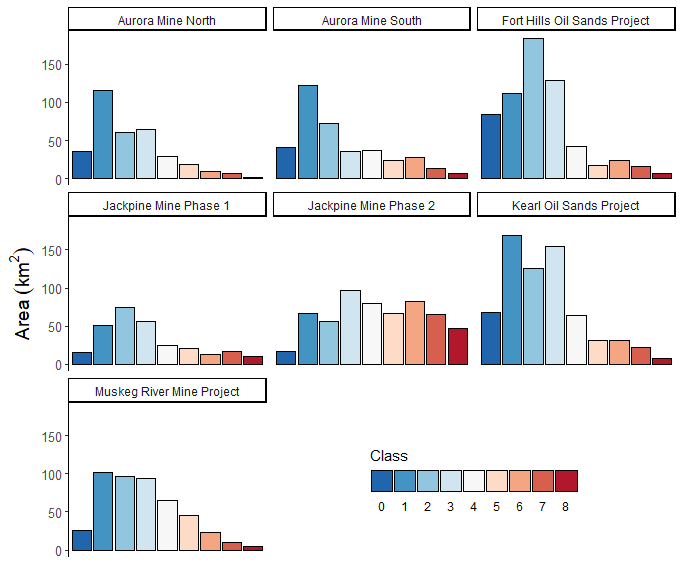
\includegraphics[width=1\linewidth]{C:/Users/mabec/Documents/R/OSM-Synthesis-YERA/./docs/pics/habitat-plots} 

}

\caption{Distribution of habitat classes in seven mining lease sites near McClelland Lake.}\label{fig:habitat-plots}
\end{figure}

\subsection{Spatially Explicit Abundance Modeling Using Satellite Remote
Sensing}\label{spatially-explicit-abundance-modeling-using-satellite-remote-sensing}

Advancements in remote sensing technologies have dramatically increased
the breadth and resolution of landcover data available for ecological
modeling purposes (Cord et al., 2013). Among these advancements has been
the availability of open-access satellite data (e.g.~Landsat,
Sentinel-1, Sentinel-2), which when combined with cloud computing power
(e.g.~through Google Earth Engine) and data science software has made
the inegration of remotely sensed data into applied ecological research
possible.

McLeod (2019) used the Yellow Rail abundance data collected throughout
the OSM (and more broadly, the Lower Athabasca Region) to build a
distribution model with landcover information directly derived from
satellite data. This information included data obtained from Sentinel-1,
Sentinel-2 (Copernicus Programme, 2017) and the Advanced Land Observing
Satellite (ALOS) Digital Elevation Model (DEM) (JAXA, 2019), which were
then processed using Google Earth Engine. A total of 15 input variables
were used in the model to predict Yellow Rail abundance, including
Anthocyanin Reflectance Index (ARI), the Normalized Difference of
Polarization (DPOL), a topographic wetness index, and a Red Edge
Inflection Point (REIP). A boosted regression tree modeling approach was
used to fit the distribution model for Yellow Rail. There are several
inherent advantages to this approach of using remotely sensed data
directly. First, it allows for avoidance of building models off prior
models (e.g.~landcover classifications), which compounds error rates
(McLeod, 2019). Additionally, the continual collection of satellite data
makes it possible to dynamically update a species distribution model
with annual, or seasonal, remotely sensed inputs to better reflect
changes within a dynamic wetland ecosystem (like those preferred by
Yellow Rail) (McLeod, 2019).

Displayed below is a subset of the predictive map, which shows the
predicted abundance of breeding Yellow Rail at a 10-m resolution in both
the eastern and western portions of the McClelland Fen Mine area. Note
that upland areas were excluded from the model's predicted area. As
McLeod (2019) explains, the predicted abundances should be interpreted
as an ordered rank where higher predictions equate to an increased
likelihood that more individual Yellow Rail are present during the
breeding season.

The potential also exists for remote sensing techniques to help quantify
water depth at survey site locations. As mentioned previously, water
depth measurements were taken by field staff during the Yellow Rail
monitoring program; however, in some cases, practical sampling
difficulties has rendered parts of this dataset incomplete.
Supplementing this information with radar data from satellites could
potentially improve habitat modeling capabilities (e.g.~Jiang et al.,
2015).

\subsection{Regional Population
Estimates}\label{regional-population-estimates}

Hedley et al (\emph{in prep}) used the results of the habitat
suitability map, combined with occupancy modeling, to produce a regional
population estimate for Yellow Rail\footnote{Note that this regional
  population estimate applies to the area covered by the habitat
  suitability map, not the OSR as a whole.}. Occupancy rates in each
habitat class (0-8) were extrapolated to the rest of the region using a
hexagon grid methodology, where a hexagon grid is simulated across the
study area and points are generated at the centroid. Two grid sizes, in
terms of distance between centroids, were chosen based on assumptions
about the detection radius of the ARUS, territory size, and territory
shape (details available in Hedley et al, \emph{in prep}): 802-m and
605-m. Once these grids were simulated across the landscape, occupancy
rate was predicted at each cell according to the habitat class at the
centroid.

Using the larger grid size, which is based on an assumed effective ARU
detection distance of 250-m, the total regional population size was
estimated to be 1,597 males. With the smaller grid size, based on a
effective detection distance of 150-m, the regional population estimate
was 2,636 males. The table below summarizes these findings.

Relative to their share of the total area (13.9\%), leased areas (both
mining and \emph{in situ}) account for a proportionally higher share of
the estimated regional population of Yellow Rails (17\%).

\section{Discussion}\label{discussion}

The boreal forest of Alberta was formerly considered an area of
secondary importance for Yellow Rails. This is no longer the case, as
bioacoustic surveys conducted in the past decade have significantly
increased the number of confirmed Yellow Rails in the OSR. It now seems
likely that this region hosts a significant proportion of the global
population of Yellow Rails.

Yellow Rails are not evenly distributed across the boreal forest, but
are concentrated in large wetland complexes. Conservation efforts should
focus on minimizing the effects of development within these important
habitats. New tools are available that can help visualize Yellow Rail
occurrence and identify breeding sites for surveys.

Placing the threat in a broader regional and global context is also
important. Regionally, surveys should be conducted in more large wetland
complexes with high predicted habitat suitability to identify new
significant breeding sites or confirm their absence. Globally, efforts
should be made to refine population estimates by synthesizing
information across known breeding hotspots in each province.

\section{References}\label{references}

Austin, J. E., \& Buhl, D. A. (2013). Relating Yellow Rail ( Coturnicops
noveboracensis ) Occupancy to Habitat and Landscape Features in the
Context of Fire. Waterbirds, 36(2), 199--213.

Bookhout, T. A., \& Stenzel, J. R. (1987). Habitat and movements of
breeding yellow rails. Wilson Bulletin, 99(3), 441--447.

Copernicus Programme. (2017). Sentinel-2 User Handbook. Retrieved
fromhttps://sentinels.copernicus.eu/web/sentinel/user-guides/document-library/-/asset\_publisher/xlslt4309D5h/content/sentinel-2-user-handbook.

Cord, A. R., Meentemeyer, R. K., Leitao, P. J., \& Vaclavik, T. (2013).
Modelling species distributions with remote sensing data: bridging
disciplinary perspectives. Journal of Biogeography, 40, 2226--2227.

COSEWIC. (2009). Assessment and Status Report on the Yellow Rail
Coturnicops noveboracensis in Canada. Committee on the Staus of
Endangered Wildlife in Canada.

Environment Canada. (2013). Management plan for the yellow rail
(Coturnicops noveboracensis) in Canada. Species at Risk Act Management
Plan Series.

Hatfield Consultants. (2008). Results of yellow rail surveys on the
Albian Muskeg River mine expansion area. Retrieved from
\url{http://www.ceaa.gc.ca/050/documents_staticpost/59539/50567/Appx2Results.pdf}.

Hedley, R., et al. (2019). Modeling the occurrence of the Yellow Rail
(Coturnicops noveboracensis), a bird species of conservation concern, in
the oil sands region of Alberta using bioacoustic survey data. \emph{in
prep}.

Jiang, H., Liu, C., Sun, X., Lu, J., Zou, C., Hou, Y., \& Lu, X. (2015).
Remote sensing reversion of water depths and water management for the
stopover site of siberian cranes at Momoge, China. Wetlands, 35(2),
369--379.

Leston, L., \& Bookhout, T. A. (2015). Yellow Rail (Coturnicops
noveboracensis), version 2.0. \url{https://doi.org/10.2173/bna.139}.

McLeod, L. (2019). Predictive Mapping of Yellow Rail (Coturnicops
noveboracensis) Density and Abundance in the Western Boreal Forest via
Ground and Satellite Remote Sensors. M.S Thesis. University of Alberta,
Edmonton, Alberta. 103 Pages.

Stenzel, J. R. (1982). Ecology of breeding yellow rails at Seney
National Wildlife Refuge. M.S. Thesis. Ohio State University, Columbus,
Ohio. 106 Pages.

Wells, J. V, \& Blancher, P. J. (2011). Global role for sustaining bird
populations. In J. V Wells (Ed.), Boreal birds in North America: A
hemispheric view of their conservation links and significance. Studies
in Avian Biology (no. 41) (pp.~7--22). Berkeley, CA: University of
California Press.


\end{document}
